% Copyright 2021 Fausto Spoto
%
% Licensed under the Apache License, Version 2.0 (the "License");
% you may not use this file except in compliance with the License.
% You may obtain a copy of the License at
%
%    http://www.apache.org/licenses/LICENSE-2.0
%
% Unless required by applicable law or agreed to in writing, software
% distributed under the License is distributed on an "AS IS" BASIS,
% WITHOUT WARRANTIES OR CONDITIONS OF ANY KIND, either express or implied.
% See the License for the specific language governing permissions and
% limitations under the License.

\documentclass[11pt]{beamer}  %% versione proiettore
%%\documentclass[11pt,handout]{beamer} %% versione stampa
\usepackage{lucidiJb-2ed}
\usepackage{mathtools}
\usepackage{relsize}

\mode<article>
{
  \usepackage{fullpage}
  \usepackage{hyperref}
}

\mode<presentation>
{
  \setbeamertemplate{background canvas}[vertical shading][bottom=red!10,top=blue!10]
  \usetheme{Course}
  \usefonttheme[onlysmall]{structurebold}
}

\subtitle{Blockchain Course}
\title{Bitcoin}
\institute{Universit\`a di Verona, Italy}
\date{October 2024}

\setbeamercovered{invisible}

\def\codesize{\smaller}
\def\<#1>{\codeid{#1}}
\newcommand{\codeid}[1]{\ifmmode{\mbox{\codesize\ttfamily{#1}}}\else{\codesize\ttfamily #1}\fi}

\begin{document}

\begin{frame}
  \titlepage
\end{frame}

\begin{frame}
  \frametitle{The internet of money}

  \begin{greenbox}{What do we expect from money}
    \begin{itemize}
    \item money should be protected from counterfeiting (\emph{legality})
    \item money should not be spent twice (\emph{uniqueness})
    \item no one can claim that my money belongs to him (\emph{ownership})
    \end{itemize}
  \end{greenbox}

  \bigskip

  Electronic money exists since decades (credit cards, online transactions)

  \bigskip

  \begin{greenbox}{}
    Bitcoin provides a \alert{fully decentralized} electronic cash system, for the first time
    (a single State cannot shut down the bitcoin network)
  \end{greenbox}

  \bigskip

  ``Bitcoin: A Peer-to-Peer Electronic Cash System'' by Satoshi Nakamoto, 2008

\end{frame}

\begin{frame}\frametitle{Reference used in this course}

  \begin{center}
    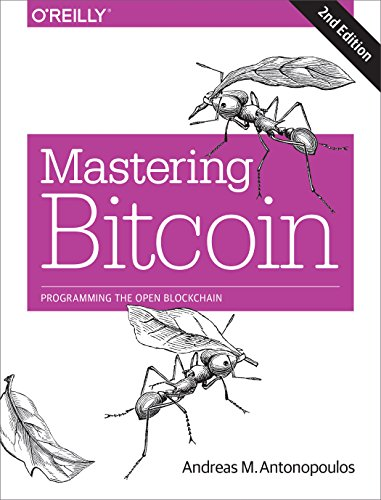
\includegraphics[scale=.35,clip=false]{pictures/mastering-bitcoin.jpg}
  \end{center}

  \begin{center}
    \url{https://github.com/bitcoinbook/bitcoinbook}
  \end{center}

\end{frame}

\begin{frame}\frametitle{Bitcoin as a web service}

  \begin{center}
    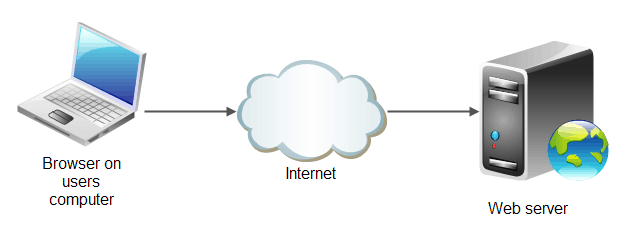
\includegraphics[scale=.3,clip=false]{pictures/web-server.png}
  \end{center}

  \medskip

  The server keeps a map (\alert{ledger}) $\mathit{user\_id}\Rightarrow\mathit{balance}$
  and accepts transactions to transfer balances

  \medskip

  Users interact through a browser (\alert{wallet}) to ask to transfer balances

  \medskip
  The server is actually a worldwide peer-to-peer (p2p) network of computers

  \begin{center}
    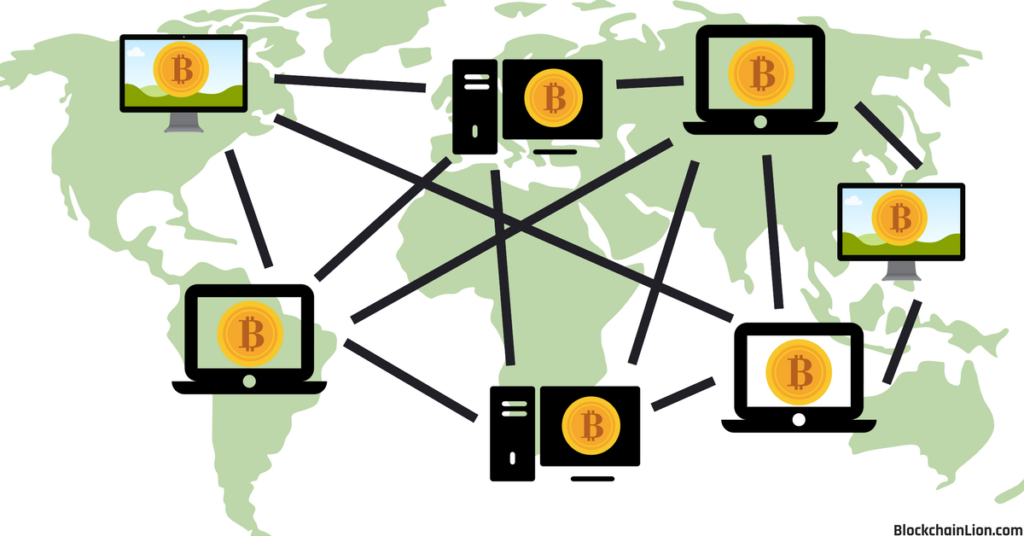
\includegraphics[scale=.13,clip=false]{pictures/distributed.png}
  \end{center}

\end{frame}

\begin{frame}\frametitle{Wallets}

  \begin{itemize}
  \item desktop wallets
  \item mobile wallets
  \item web wallets
  \item hardware wallets
  \item paper wallets
  \end{itemize}
  
\end{frame}

\begin{frame}\frametitle{Mobile wallets}

  At the first start-up, a bitcoin address is created for you, then transactions
  from/to that address are tracked:

  \begin{center}
    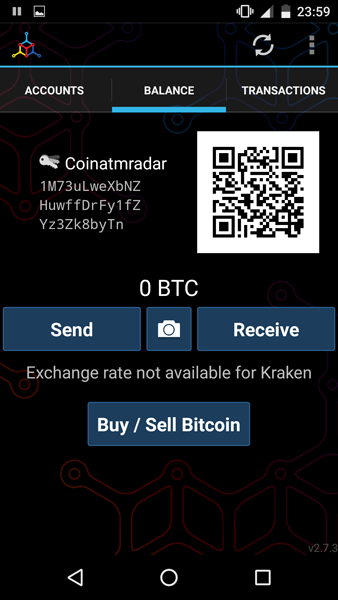
\includegraphics[scale=0.27,clip=false]{pictures/bitcoin-wallet.png}
  \end{center}

  The \alert{address} can be seen as our IBAN. Its creation
  is a local operation that does not do anything on the network: fully anonymous

\end{frame}

\begin{frame}\frametitle{Address creation}

  When Alice's wallet starts for the first time:

  \begin{enumerate}
  \item it generates a finite sequence of bits through a secure random generator
    (a secret private key)
  \item it computes the bitcoin address as an abstraction of the private key
    (hashing)
  \item it shows the bitcoin address as an alphanumeric string and as a picture (QR code)
  \item \alert{the address is not sensitive information}: Alice can publish it in her web page
  \item \alert{the private key is sensitive information}: Alice keeps it secret
    \begin{itemize}
    \item a hardware wallet stores it in its internal memory
    \item a desktop wallet stores it in Alice's computer's file system (!)
    \item a mobile wallet stores it in Alice's phone (!!!)
    \item a web wallet stores it at a third-party service (!!!!!!!)
    \end{itemize}
  \end{enumerate}
\end{frame}

\begin{frame}\frametitle{Random generators}

  \begin{redbox}{Cryptographically-secure random generators}
    Private keys should be generated by using a cryptographically-secure
    random generator, or otherwise keys might not really be randomly
    spread and might be more easily guessed
  \end{redbox}

  \medskip

  \begin{greenbox}{In Java}
    \texttt{java.security.SecureRandom}, not \texttt{java.util.Random}
  \end{greenbox}

  \medskip

  \begin{greenbox}{}
    The generation of private keys does not require any
    centralized service and occurs completely outside the blockchain,
    offline. The probability of computing an already used key is negligeable
  \end{greenbox}

\end{frame}

\begin{frame}\frametitle{Alice recharges her wallet}
  \begin{itemize}
  \item she asks a friend to send bitcoins at her address
  \item or meets a bitcoin seller in person
  \item or earns bitcoin by working
  \item or uses a bitcoin ATM
  \item or uses a bitcoin currency exchange company
  \end{itemize}

  \bigskip

  \begin{greenbox}{What is the price?}
    It is not set by the computer network! It's a social
    agreement, the average of the last sell operations.
    You can look online for it
  \end{greenbox}

\end{frame}

\begin{frame}\frametitle{The recharge transaction}

  \begin{enumerate}
  \item Joe (the seller) specifies in his wallet Alice's bitcoin address
    as destination (or scans Alice's QR code with his mobile)
  \item Joe signs a transaction (a sequence of bits),
    with his private key, stating: \emph{``I acknowledge
    to send X bitcoins from my address to Alice's destination address''}
  \item Joe's wallet broadcasts the signed transactions
    to one (or more) servers of the bitcoin network
  \item the network spreads the information and eventually the transaction is cleared
    (in $10$ minutes or more)
  \item Alice's wallet polls the bitcoin network for a transaction having
    Alice's address as destination and updates the balance on the screen
    accordingly (\alert{confirmation})
  \end{enumerate}

\end{frame}

\begin{frame}\frametitle{The spend transaction}

  Alice's wallet is now recharged and she wants to buy a coffee at Bob's coffee shop:

  \begin{enumerate}
  \item Alice's wallet signs, with her private key, a transaction
    (a sequence of bits) stating: \emph{``I acknowledge to send Y bitcoins from Alice's address
    to Bob's destination address''} (some metadata can be added)
  \item the transaction is broadcast to one (or more) nodes of the
    bitcoin network and eventually cleared
  \item Alice's wallet polls the bitcoin network for a transaction having
    her address as source and updates the balance on the screen
    accordingly (\alert{confirmation})
  \end{enumerate}

  \medskip
  See it online:
  {\scriptsize\url{https://explorer.btc.com/btc/transaction/0627052b6f28912f2703066a912ea577f2ce4da4caa5a5fbd8a57286c345c2f2}}

\end{frame}

\begin{frame}\frametitle{Offline signing}

  \begin{greenbox}{}
    For extreme security, transactions might be signed offline,
    on an \emph{airgapped} computer, so that private keys are not
    in memory of any connected computer
  \end{greenbox}

  \bigskip

  \begin{center}
    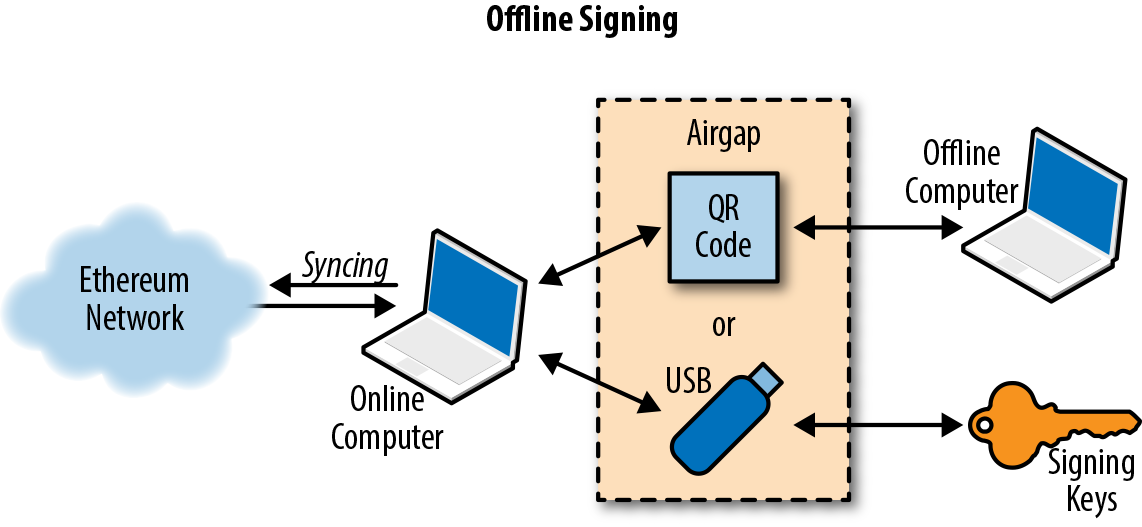
\includegraphics[width=\textwidth,clip=false]{pictures/offline_signing.png}
  \end{center}

\end{frame}

\begin{frame}\frametitle{The transaction}

  \begin{center}
    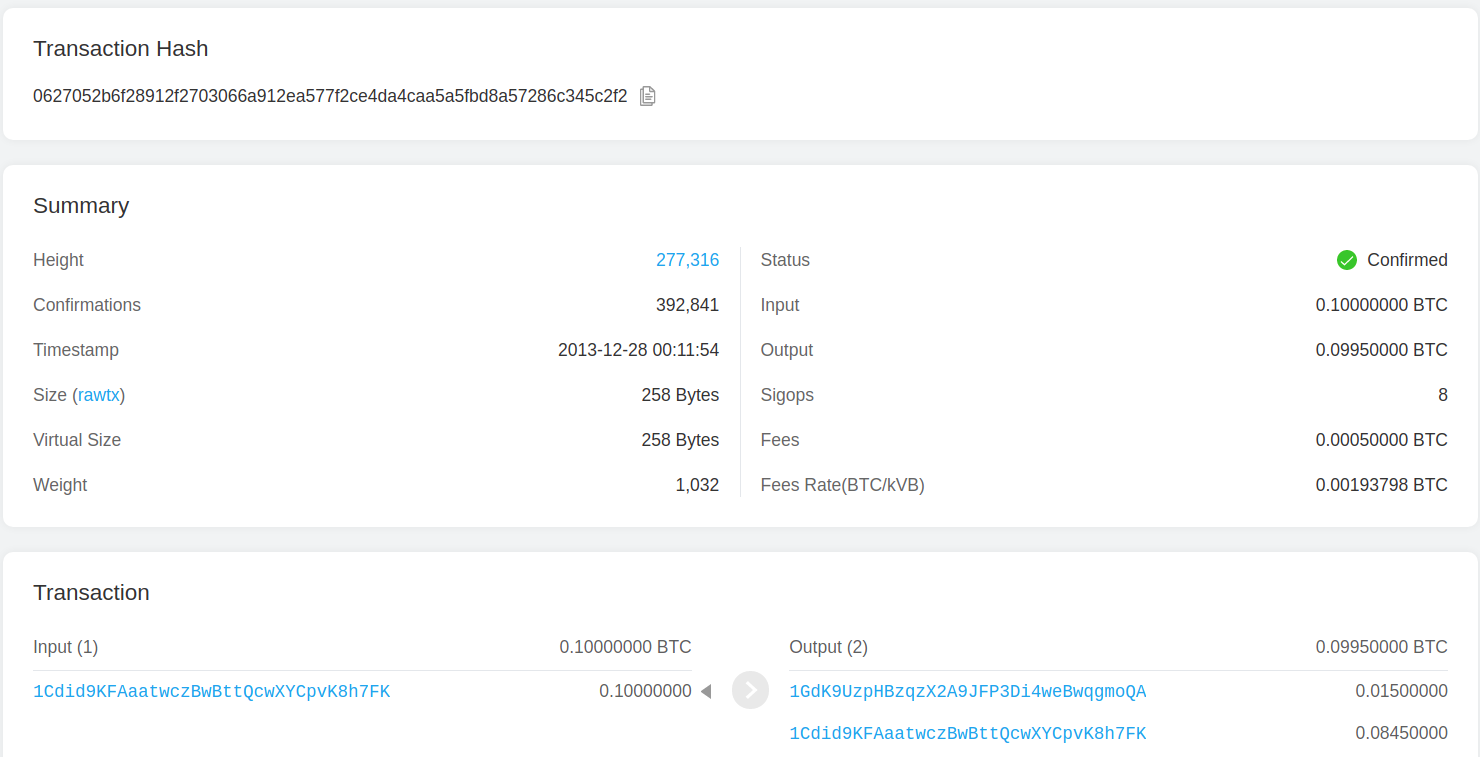
\includegraphics[scale=0.23,clip=false]{pictures/bitcoin-spend.png}
  \end{center}

\end{frame}

\begin{frame}\frametitle{Transactions form a chain, outputs can be change}

  \begin{center}
    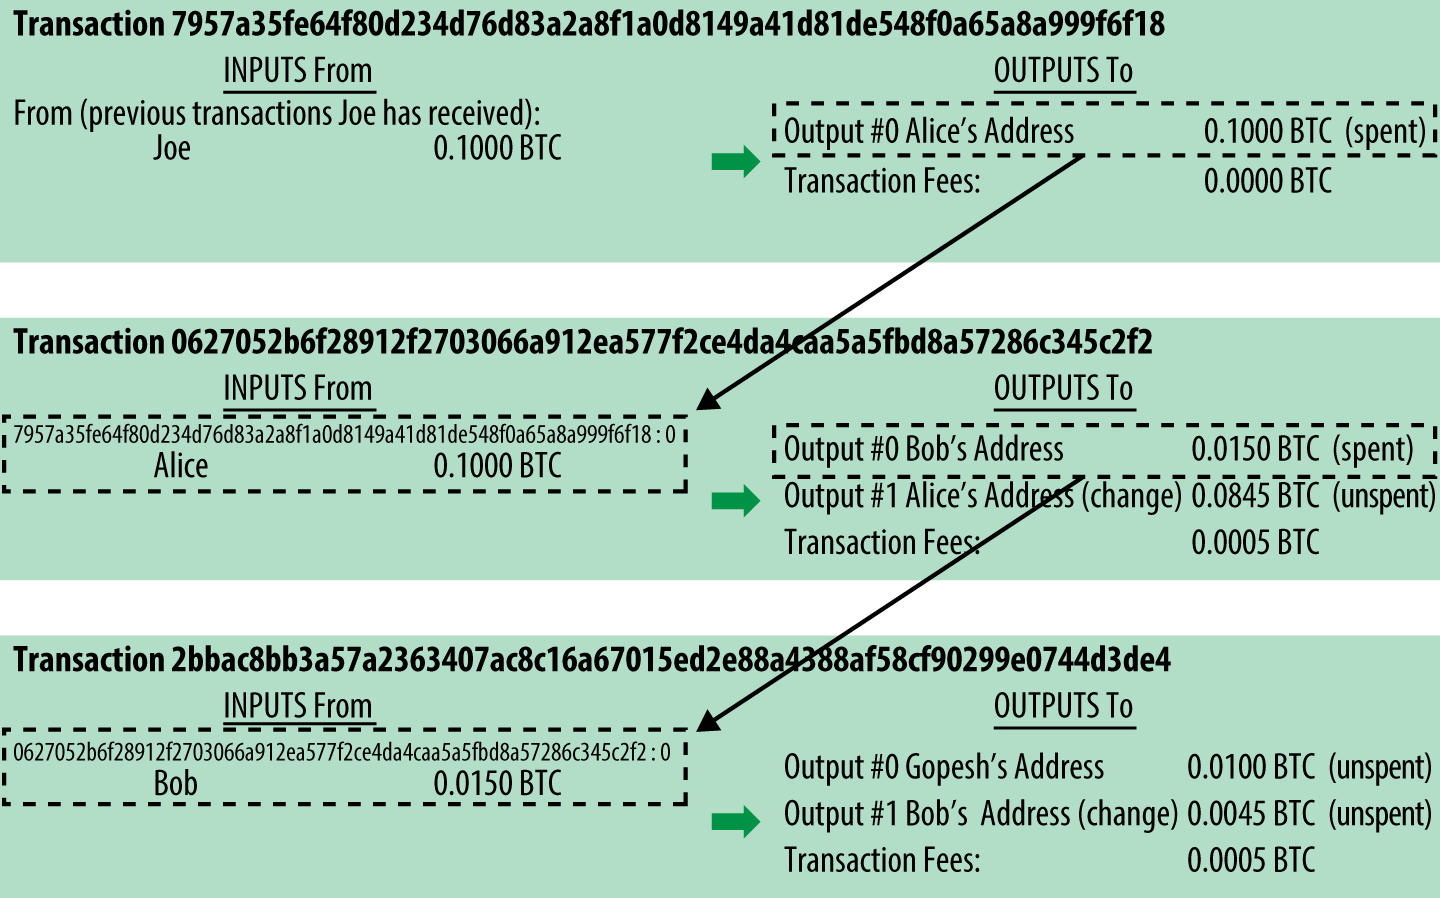
\includegraphics[scale=0.23,clip=false]{pictures/mbc2_0204.png}
  \end{center}

\end{frame}

\begin{frame}\frametitle{Typical transaction: pay somebody and gets the change}

  \begin{center}
    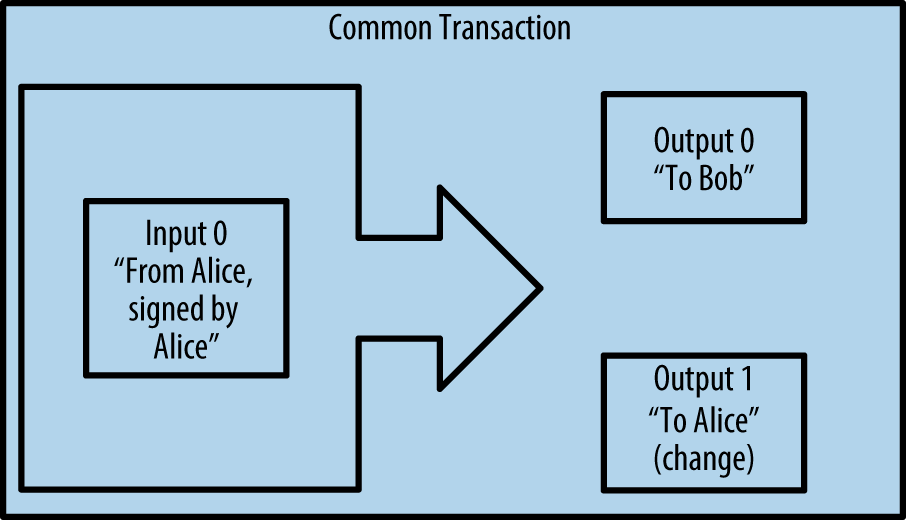
\includegraphics[scale=1.2,clip=false]{pictures/mbc2_0205.png}
  \end{center}

\end{frame}

\begin{frame}\frametitle{Typical transaction: aggregate small notes into a larger one}

  \begin{center}
    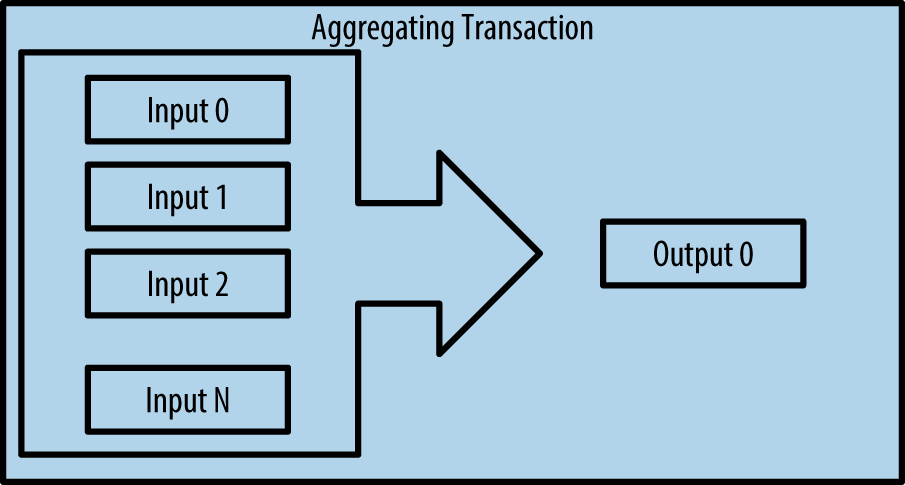
\includegraphics[scale=1.2,clip=false]{pictures/mbc2_0206.png}
  \end{center}

\end{frame}

\begin{frame}\frametitle{Typical transaction: distribution}

  \begin{center}
    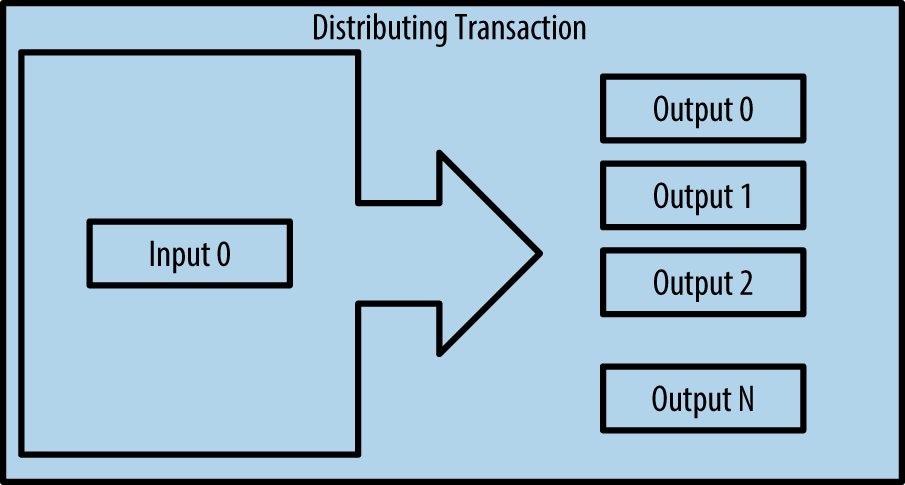
\includegraphics[scale=1.2,clip=false]{pictures/mbc2_0207.png}
  \end{center}

\end{frame}

\begin{frame}\frametitle{A DAG of transactions}

  \begin{center}
    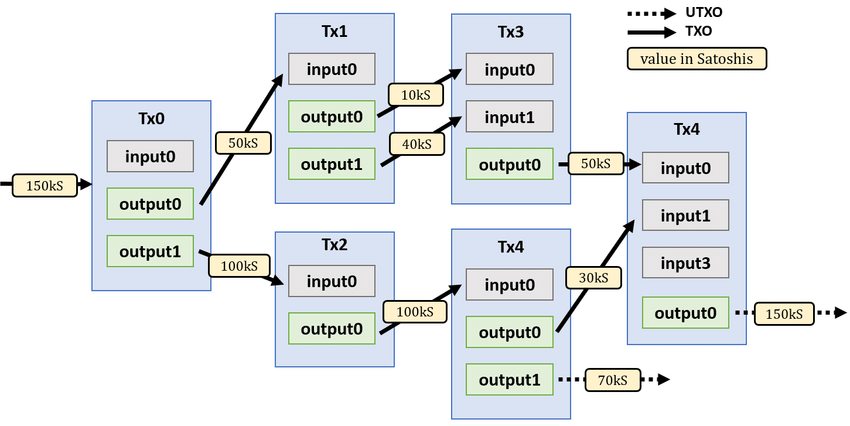
\includegraphics[width=\textwidth,clip=false]{pictures/bitcoin-dag.png}
  \end{center}

\end{frame}

\begin{frame}\frametitle{How Alice's wallet prepares a transaction}

  \begin{enumerate}
  \item Alice's wallet keeps a list of all known unspent outputs for the address
    of Alice
    \begin{itemize}
    \item if it does not know it, it can query the bitcoin network through an API
    \end{itemize}
  \item the wallet selects a subset $\mathit{inputs}$ of the unspent outputs, enough to cover
    the $\mathit{amount}$ of the transaction
    \begin{itemize}
    \item any strategy can be applied here
    \end{itemize}
  \item the wallet specifies an output for the destination address of the transaction
    and the $\mathit{amount}\ge 0$ sent to that output
  \item the wallet specifies a second output, normally Alice's address itself, and the
    $\mathit{change}\ge 0$ sent back to Alice
  \item the difference
    \[
    \mathit{fee}=\sum\mathit{inputs}-\mathit{amount}-\mathit{change}\ge 0
    \]
    is the network's reward (and protection) for processing the transaction
  \end{enumerate}

\end{frame}

\begin{frame}\frametitle{How Alice sends the transaction}

  \begin{enumerate}
  \item Alice's wallet sends the bytes of the transaction to a node of the
    bitcoin p2p network
    \begin{itemize}
    \item or it can store it on a removable memory support and another device
      will send it
    \end{itemize}
  \item the transaction gets forwarded among all peers (flooding)
  \item the wallet of the destination will very soon see a transaction
    for its address and can assume that it will eventually be processed
    (\alert{unconfirmed transaction})
  \item eventually, around $10$ minutes later,
    the transaction will be processed by the network and
    the wallet of the destination will notice that (\alert{confirmed transaction})
  \item after some time, around one hour, the transaction can be considered
    as definitively processed (\alert{finalized transaction})
  \end{enumerate}

  Merchants can wait for 3, 4 or 5 before handling over the good,
  depending on the relevance of the transaction

\end{frame}

\begin{frame}\frametitle{Miners and Rewards}

  \begin{greenbox}{Miners are (some) nodes of the bitcoin network. They receive, forward
      and aggregate transactions into collectors, called \alert{blocks}}
    When a node creates a new block, it has the right to tag the block
    with a bitcoin address $\mu$, called the \alert{miner}'s address:
    \begin{itemize}
    \item the fees $\phi_1\cdots\phi_n$ of the $n$ transactions in the block go to $\mu$
    \item some amount of money $\iota$ is created out of thin air and goes to $\mu$
    \end{itemize}
  \end{greenbox}

  \bigskip

  \begin{greenbox}{}
    Typically, $\mu$ belongs to the person/organization who owns the machine that runs the node
  \end{greenbox}

  \bigskip

  \begin{greenbox}{}
    $\iota$ is the \alert{inflation}: it is computed through a fixed algorithm that makes it decrease with the time
    and will eventually reach $0$, the day when 21,000,000 total bitcoins will be mined
    \begin{itemize}
    \item[$\Rightarrow$] bitcoin is deflationary
    \end{itemize}
  \end{greenbox}

\end{frame}

\begin{frame}\frametitle{Bitcoin supply over the years}

  \begin{center}
    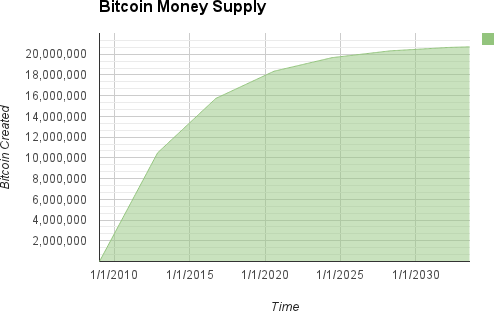
\includegraphics[width=\textwidth,clip=false]{pictures/mbc2_1001.png}
  \end{center}

\end{frame}

\begin{frame}\frametitle{How miners work}

  \begin{enumerate}
    \item Each miner listens the p2p network for new transactions and stores them in a
      temporary area called mempool
    \item when enough new transactions are available in the mempool, it selects some of them
      \begin{itemize}
      \item typically, it selects those with the largest fees, but any other choice is fine: different miners can use different strategies
      \end{itemize}
    \item it builds a new block (\alert{mining}):
      \begin{itemize}
      \item it adds the selected transactions
      \item it adds a special \alert{coinbase transaction} with no inputs, whose only output is $\mu$
        and whose amount is $\iota+\sum_{i=1}^n\phi_i$
      \item it tags the block with a reference to the previous block
      \item it tags the block with its own miner's address $\mu$
      \item it tags the block with a nonce computed by solving an expensive puzzle
      \item if no other miner has been faster, it forwards the new block to all its peers
      \end{itemize}
  \end{enumerate}
\end{frame}

\begin{frame}\frametitle{Fees}

  \begin{center}
    \url{https://bitcoinfees.net}
  \end{center}

  \bigskip
  \begin{greenbox}{For example}
    \begin{itemize}
    \item if I want a transaction processed in one hour at most, I must offer $5.41$ Satoshis per virtual byte
    \item a simple transaction is in average $140$ virtual bytes long
    \item a BTC is $60000$ euros worth (as of today)
    \end{itemize}
    \begin{center}
      $\Rightarrow$ I must offer $\frac{5.41 \cdot 140 \cdot 60000}{10^7}=0.45$ euros as fee
    \end{center}
  \end{greenbox}

  \bigskip
  \begin{redbox}{}
    \begin{center}
      The size, not the value of the transaction is relevant!
    \end{center}
  \end{redbox}

\end{frame}

\begin{frame}\frametitle{Block's height, depth and confirmations}

  \begin{center}
    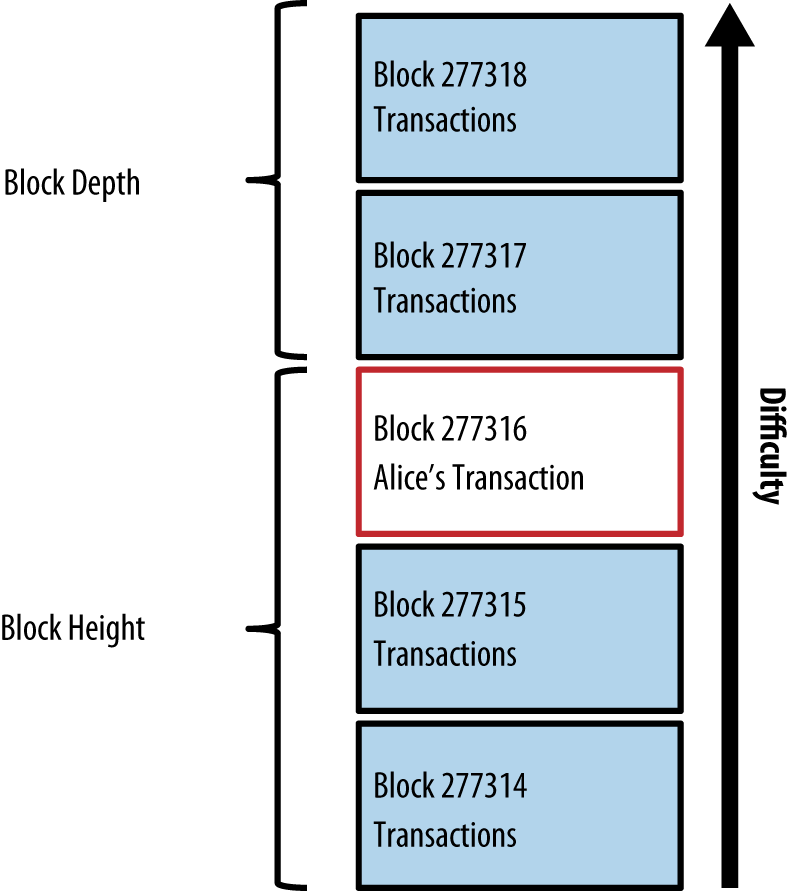
\includegraphics[scale=1,clip=false]{pictures/mbc2_0209.png}
  \end{center}

\end{frame}

\begin{frame}\frametitle{Cryptography}

  \begin{greenbox}{Bitcoin uses cryptography for many goals}
    \begin{description}
      \item[Hashing]
        \begin{itemize}
        \item for synthetic represention of very long information (compaction)
        \item for machine-independent pointers to data structures (reference)
        \item for solving a mathematical puzzle (mining)
        \end{itemize}
        \bigskip
      \item[Signature]
        \begin{itemize}
        \item to prove the identity of the sender of transactions (witness)
        \end{itemize}
    \end{description}
  \end{greenbox}

  \bigskip

  \begin{redbox}{}
    Bitcoin doesn't use cryptography to hide data
    (everybody sees everything)
  \end{redbox}

\end{frame}

\begin{frame}\frametitle{Cryptographic hash functions}

  \begin{greenbox}{}
    A \alert{hash function} maps data of arbitrary size to data of fixed size
  \end{greenbox}

  \begin{center}
    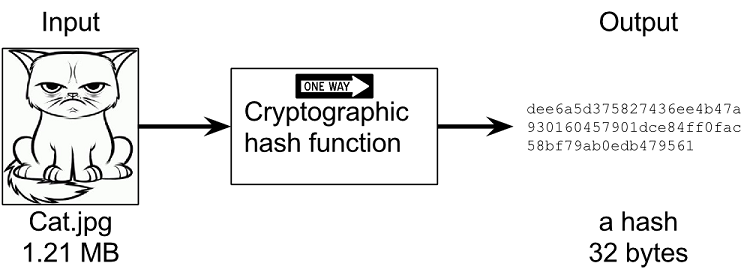
\includegraphics[scale=0.38,clip=false]{pictures/hashing.png}
  \end{center}

  \begin{greenbox}{Cryptographic hash function}
    \begin{enumerate}
    \item deterministic
    \item verifiable (in linear time)
    \item non-correlated (small change of input $\Rightarrow$ extensive change of hash)
    \item irreversible (\emph{one-way})
    \item collision-protected: difficult to compute two inputs with same hash
    \end{enumerate}
  \end{greenbox}
  
\end{frame}

\begin{frame}\frametitle{Asymmetric encryption}

  \begin{center}
    Secure random generator $\Rightarrow$ private key $\xRightarrow[]{\text{ECM}}$ public key
  \end{center}

  Ellyptic Curve Multiplication (ECM) is an abstraction or hashing algorithm
  
  \begin{center}
    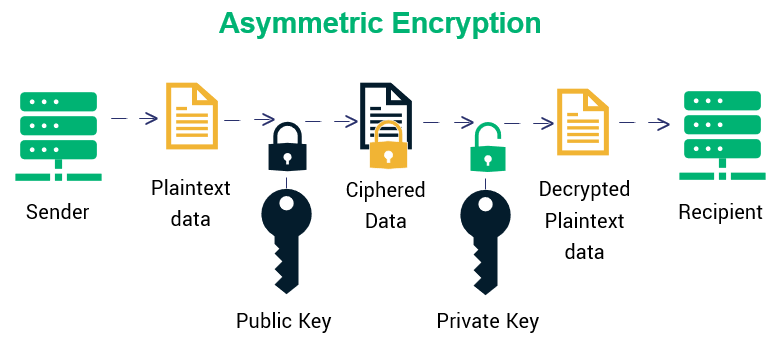
\includegraphics[scale=0.26,clip=false]{pictures/asymmetric-encryption.png}
  \end{center}

\end{frame}

\begin{frame}\frametitle{But the keys can be swapped!}

  \begin{center}
    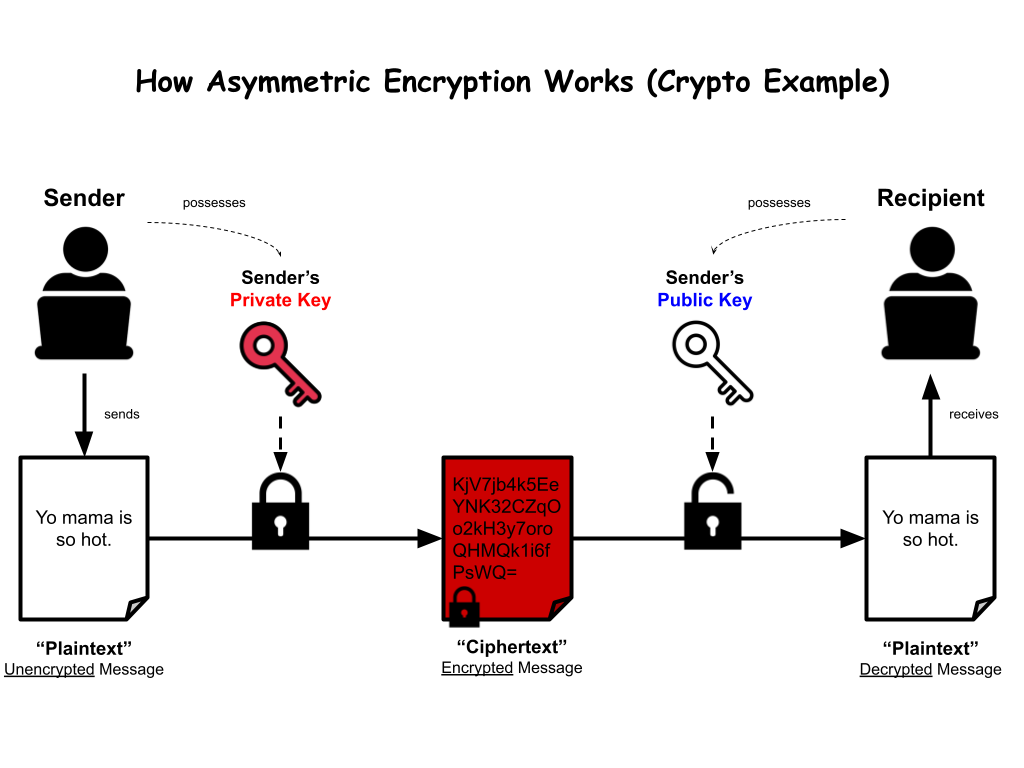
\includegraphics[scale=0.3,clip=false]{pictures/asymmetric-encryption-swapped.png}
  \end{center}

\end{frame}

\begin{frame}\frametitle{Digital signature}

  \begin{center}
    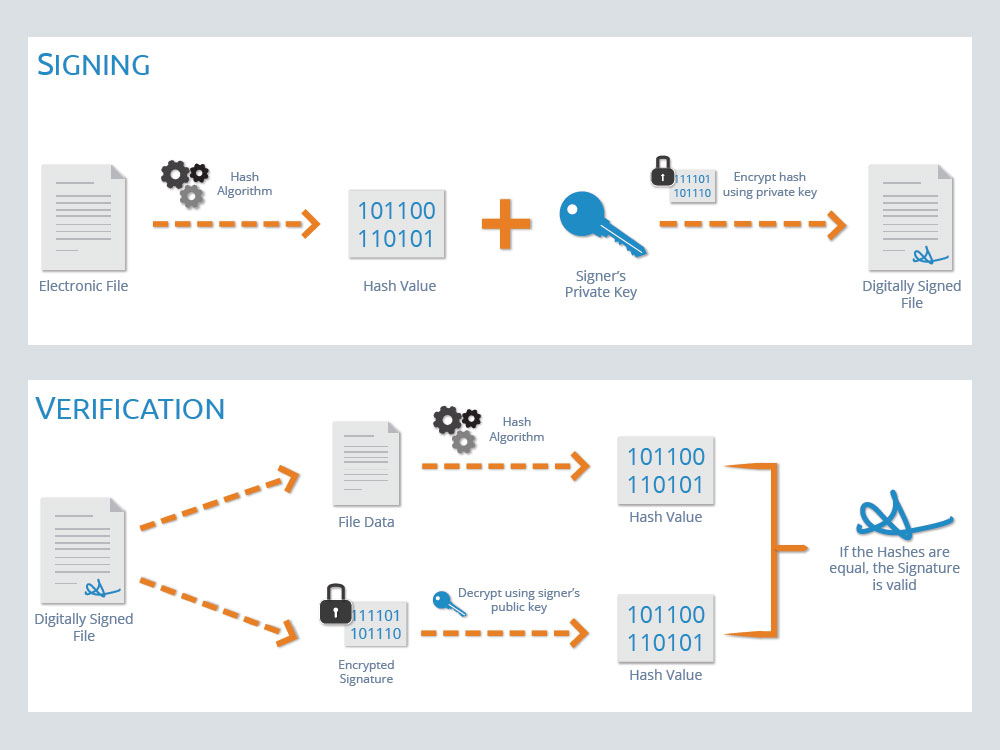
\includegraphics[scale=0.3,clip=false]{pictures/digital-signatures.jpg}
  \end{center}

\end{frame}

\begin{frame}\frametitle{Bitcoin addresses}

  \begin{itemize}
  \item private key: $256$ bits ($32$ bytes)
  \item public key: $256$ bits
  \item bitcoin address: $160$ bits ($20$ bytes \emph{ie.}, $40$ hex digits)
  \end{itemize}

  \begin{center}
    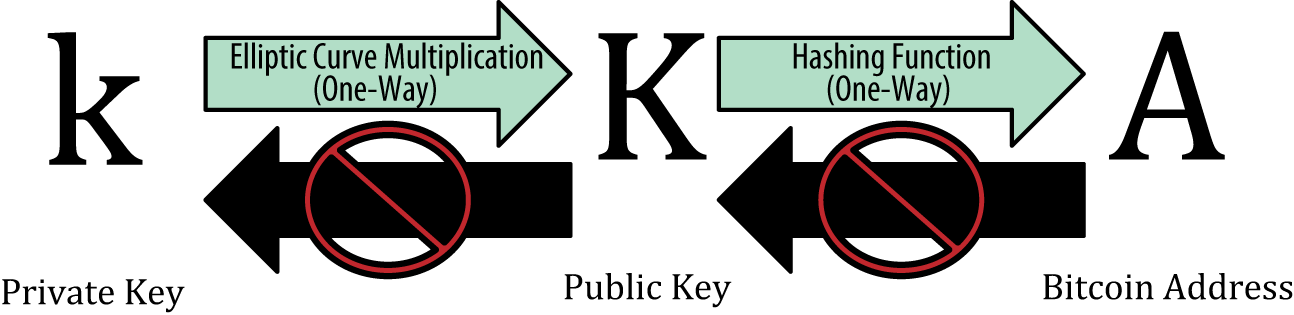
\includegraphics[scale=1,clip=false]{pictures/mbc2_0401.png}
  \end{center}

  \[A=\mathit{RIPEMD160}(\mathit{SHA256}(K))\]

\end{frame}

\begin{frame}\frametitle{Base58 representation of addresses}

  \begin{center}
    $40$ hex digits is too long!
  \end{center}

  \begin{greenbox}{Base58}
    A representation of natural numbers in base $58$, using the following
    symbols for the $58$ digits:

    \texttt{123456789ABCDEFGHJKLMNPQRSTUVWXYZabcdefghijkmnopqrstuvwxyz}

  \end{greenbox}

  \begin{center}
    $28$ Base58 digits are enough to cover $40$ hex digits
  \end{center}

\end{frame}

\begin{frame}\frametitle{Base58Check adds a checksum}

  \begin{center}
    Base58 addresses are too easy to spell wrongly!
  \end{center}

  \begin{center}
    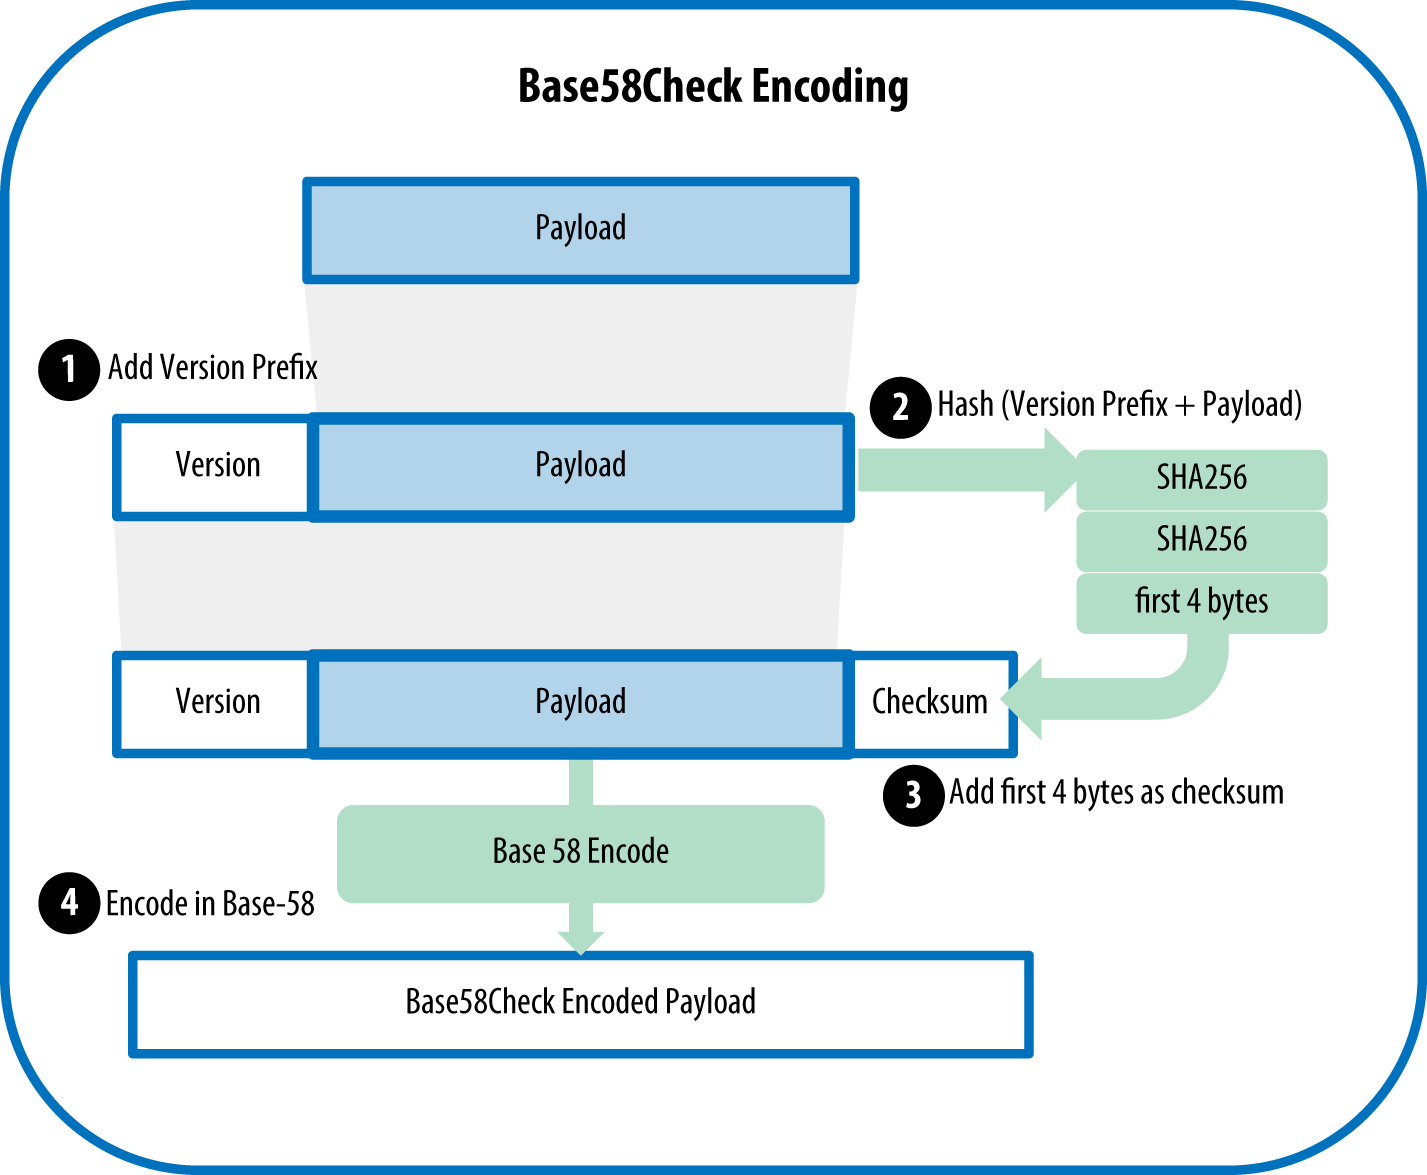
\includegraphics[scale=0.6,clip=false]{pictures/mbc2_0406.png}
  \end{center}

  \begin{center}
    $34$ Base58Check digits are enough for a bitcoin address
  \end{center}

\end{frame}

\begin{frame}\frametitle{Put it all together}

  \begin{center}
    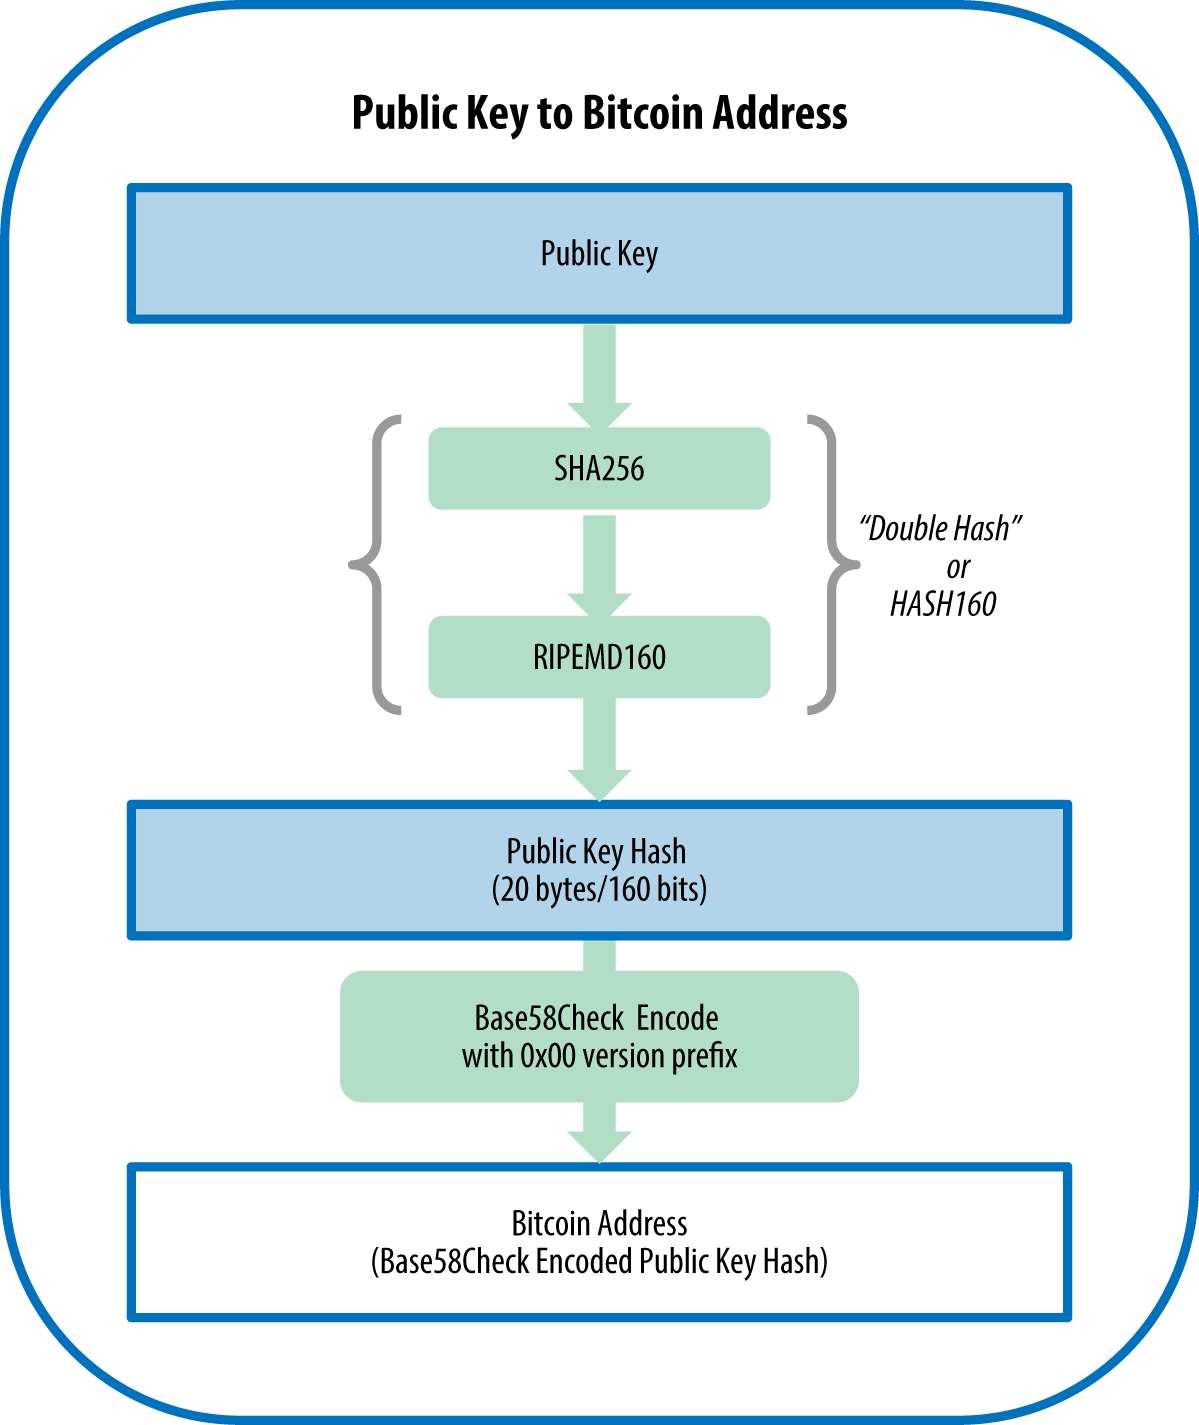
\includegraphics[scale=0.52,clip=false]{pictures/mbc2_0405.png}
  \end{center}

  \begin{center}
    Public key: {\scriptsize\texttt{0202a406624211f2abbdc68da3df929f938c3399dd79fac1b51b0e4ad1d26a47aa}}\\
    Address: \texttt{1PRTTaJesdNovgne6Ehcdu1fpEdX7913CK}
  \end{center}

\end{frame}

\begin{frame}\frametitle{Libraries}

  \begin{greenbox}{There are many libraries for computing private and public keys}
  \begin{itemize}
  \item OpenSSL (\url{https://www.openssl.org})
  \item libsecp256k1 (\url{https://github.com/bitcoin-core/secp256k1})
  \item bitcoinj (\url{https://bitcoinj.org})
  \item Bouncy Castle (\url{https://www.bouncycastle.org})
  \end{itemize}
  \end{greenbox}

\end{frame}

\begin{frame}\frametitle{Vanity addresses}

  \begin{greenbox}{Alice wants a bitcoin address whose first letters are ``Love''}
  \begin{center}
    \texttt{1\alert{Love}BPzzD72PUXLzCkYAtGFYmK5vYNR33}
  \end{center}
  \end{greenbox}

  \bigskip

  \begin{itemize}
  \item vanity addresses can only be found by brute-force computation
  \item realistic up to $7$ characters
  \item vanity addresses are typically recycled for many transactions, since
    they are hard to find
    \begin{description}
      \item[$\Rightarrow$] reduced security
    \end{description}
  \end{itemize}

  \bigskip

  \begin{center}
    \url{https://vanitypool.appspot.com/}
  \end{center}

\end{frame}

\begin{frame}
  \frametitle{Wallets}

  \begin{greenbox}{}
    A wallet is a software \alert{application} that keeps track of keys.
    It creates and broadcasts transactions signed with those keys
  \end{greenbox}

  \bigskip

  \begin{greenbox}{}
    A wallet is the \alert{file} where key pairs are stored
  \end{greenbox}

  \bigskip
  \begin{greenbox}{The simplest: a nondeterministic wallet (a bunch of keys, Type-0)}
    \begin{center}
      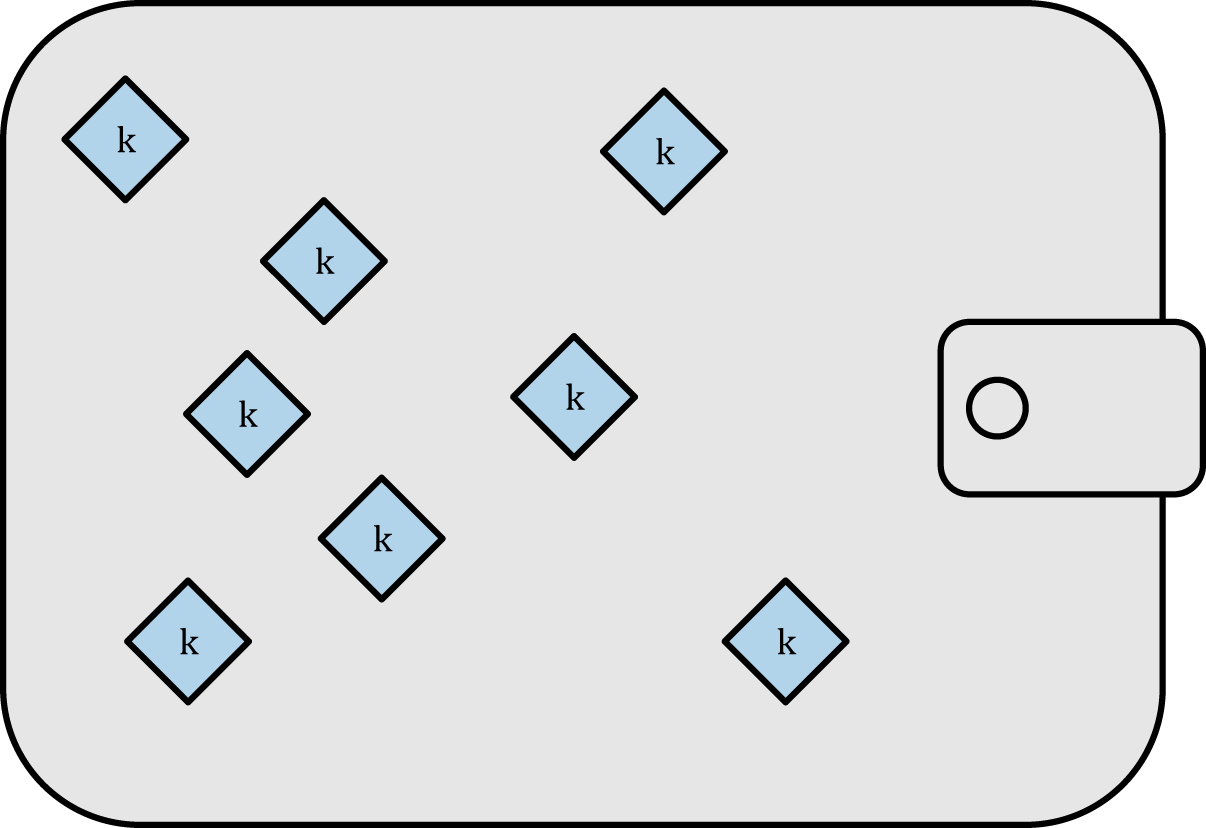
\includegraphics[scale=0.45,clip=false]{pictures/mbc2_0501.png}
    \end{center}
    Hard to backup!
  \end{greenbox}

\end{frame}

\begin{frame}\frametitle{Deterministic wallets (BIP-32, seeded, Type-1)}

  \begin{greenbox}{Streams of keys}
    They store just a seed, from which streams of keys are derived:
    \begin{itemize}
    \item only the seed must be stored, backed up and kept private
    \item different streams can be allocated for different goals or to distinct enterprise departments
    \end{itemize}
  \end{greenbox}

  \medskip

  \begin{center}
    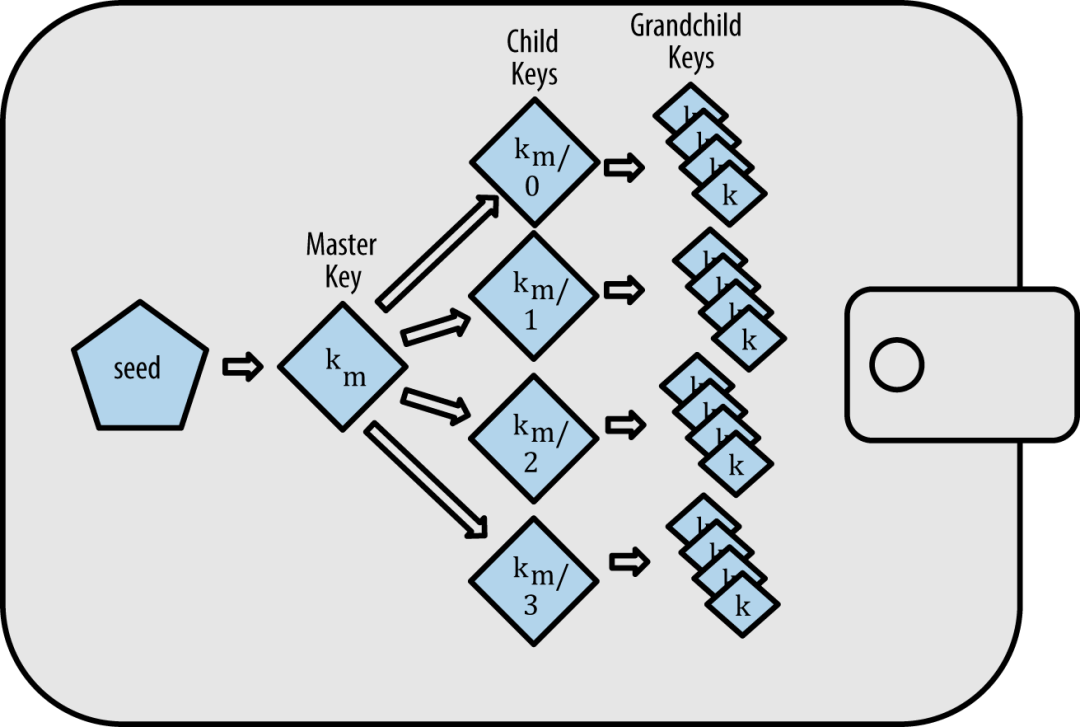
\includegraphics[scale=0.73,clip=false]{pictures/hd-wallet.png}
  \end{center}

\end{frame}

\begin{frame}\frametitle{Encoding the seed as mnemonic code words (BIP-39)}

  \begin{greenbox}{What is simpler and less error-prone to remember and backup?}
    \begin{center}
      \texttt{0C1E24E5917779D297E14D45F14E1A1A}\\
      \mbox{}\\
      or rather\\
      \mbox{}\\
      \texttt{army van defense carry jealous true}\\
      \texttt{garbage claim echo media make crunch}
    \end{center}
  \end{greenbox}

\end{frame}

\begin{frame}\frametitle{Generation of the mnemonic words}

  \begin{center}
    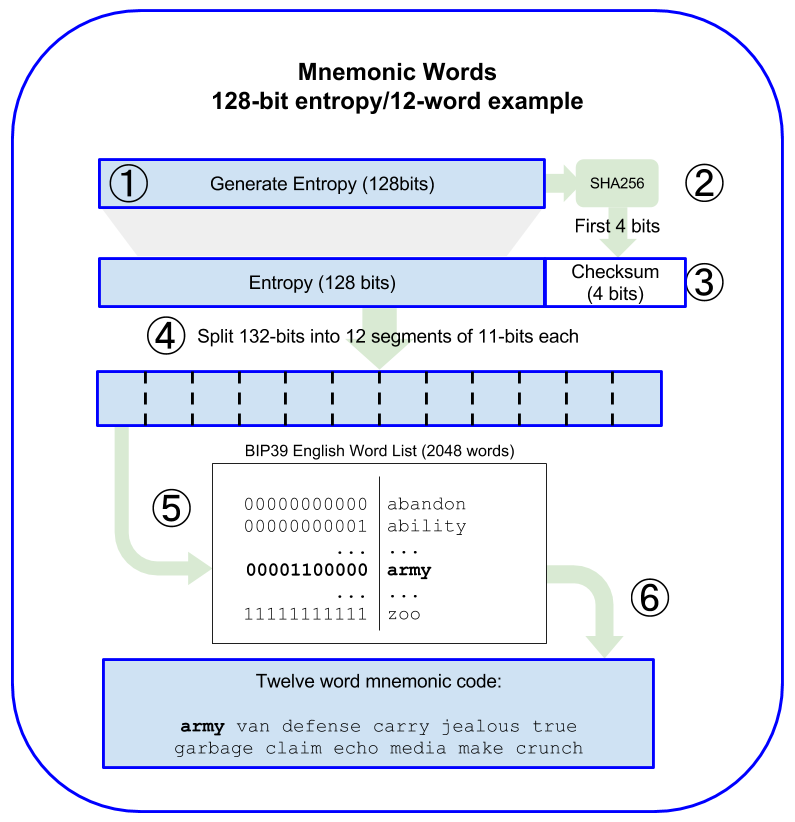
\includegraphics[scale=0.27,clip=false]{pictures/entropy-to-mnemonic.png}
  \end{center}

\end{frame}

\begin{frame}\frametitle{Generation of the seed from the mnemonic words}

  \begin{center}
    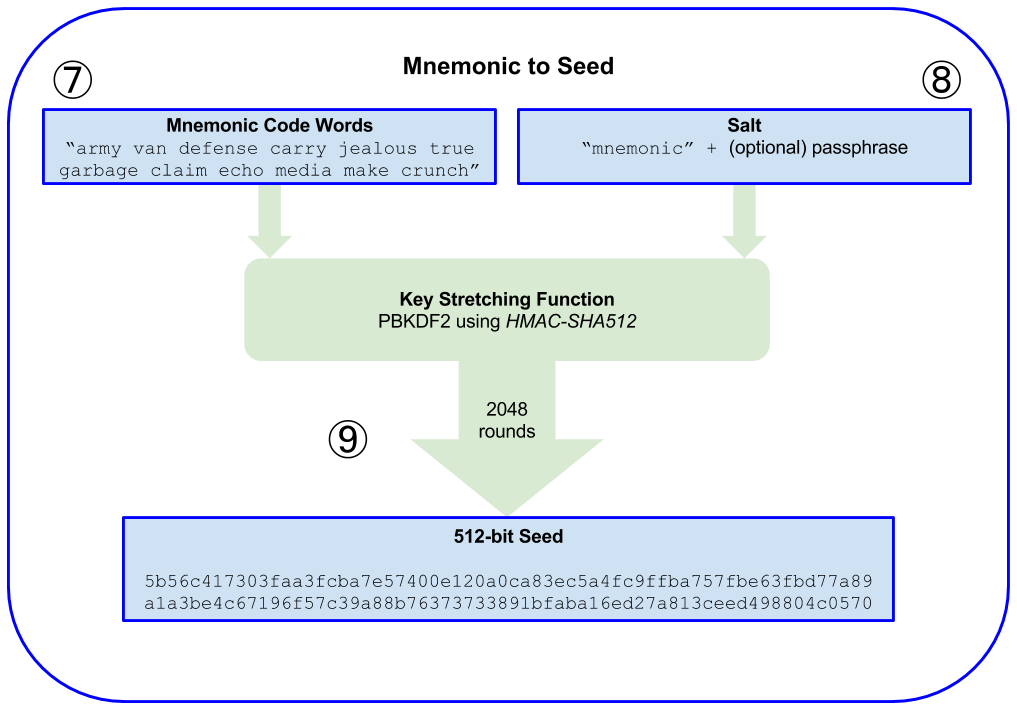
\includegraphics[scale=0.27,clip=false]{pictures/mnemonic-to-seed.png}
  \end{center}

\end{frame}

\begin{frame}\frametitle{Practical considerations}

  \begin{itemize}
  \item keep the mnemonic on paper, never in digital form
  \item memorize the passphrase
  \item let somebody else memorize the passphrase (at least, before you die)
  \item hint towards a wrong passphrase, leading to a \emph{duress wallet}
  \end{itemize}

  \bigskip

  \begin{redbox}{There are no \emph{wrong} passphrases}
    Every passphrase leads to some wallet, which unless previously used will be empty
  \end{redbox}

\end{frame}

\begin{frame}\frametitle{Parent-to-child key derivation (BIP-32)}

  \begin{itemize}
  \item there is an algorithm to derive private child keys from private parent keys
  \item there is an algorithm to derive public child keys from public parent keys
    \begin{itemize}
    \item ideal for storing only public keys in a cloud server
    \end{itemize}
  \item the derivation can be \emph{hardened}, so that
    the leak of a single private key does not allow one to reconstruct
    the other private keys
  \end{itemize}

  \begin{center}
    \begin{tabular}{ll}
      HD path & Key described \\\hline
      \<m/0> & The first (\<0>) child private key of the master private key (\<m>) \\
      \<m/0/0> & The first child private key of the first child (\<m/0>) \\
      \<m/0'/0> & The first normal child of the first \emph{hardened} child (\<m/0'>) \\
      \<m/1/0> & The first child private key of the second child (\<m/1>) \\
      \<M/23/17/0/0> & The first child public key of the first child\\
                     & of the 18th child of the 24th child
    \end{tabular}
  \end{center}
\end{frame}

\begin{frame}\frametitle{Giving structure to the key hierarchy (BIP-44)}

  \begin{center}
    \<[m|M]/purpose'/coin\_type'/account'/change/address\_index>
  \end{center}

  \bigskip

  \begin{greenbox}{}
    The value of \<purpose> is fixed to \<44>.
    For Bitcoin, \<coin\_type> is fixed to \<0> (while it is \<60> for
    Ethereum, with \<change> fixed to \<0>):
    \begin{center}
      \<[m|M]/44'/0'/account'/[0|1]/address\_index>
    \end{center}

    \begin{center}
      \begin{tabular}{ll}
        HD path & Key described \\\hline
        \<M/44'/0'/0'/0/2>  & The 3rd receiving public key\\
                            & for the primary bitcoin account\\
        \<M/44'/0'/3'/1/14> & The 15th change-address public key\\
                            & for the 4th bitcoin account\\
        \<M/44'/60'/0'/0/2> & The third public key for the primary\\
                            & Ethereum account\\
        \<m/44'/2'/0'/0/1>  & The second private key for the primary\\
                            & Litecoin account
      \end{tabular}
    \end{center}
  \end{greenbox}
\end{frame}

\begin{frame}\frametitle{The transaction, again}

  \begin{center}
    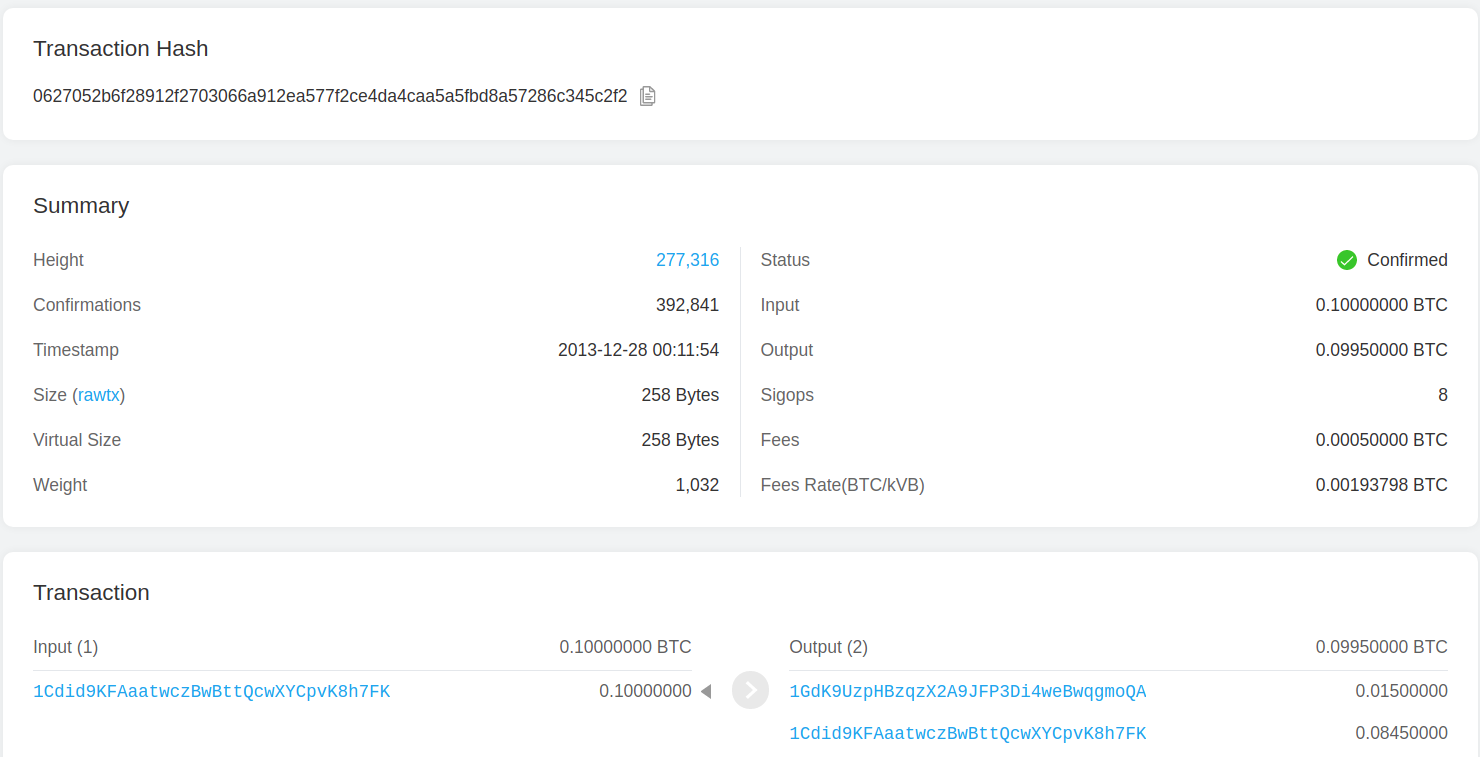
\includegraphics[scale=0.23,clip=false]{pictures/bitcoin-spend.png}
  \end{center}

\end{frame}

\begin{frame}[fragile]\frametitle{The real transaction}

  \begin{center}
    no coins, no senders, no recipients, no balances, no accounts, no addresses
  \end{center}

  {\scriptsize\begin{alltt}
\{
  "vins": [
    \{
      "txid": "7957a35fe64f80d234d76d83a2a8f1a0d8149a41d81de548f0a65a8a999f6f18",
      "vout": 0,
      "unlock": "3045022100884d142d86652a3f47... 0484ecc0d46f..."
    \}
  ],
  "vouts": [
    \{
      "value": 0.01500000,
      "lock": "DUP HASH160 ab68025513c3dbd2f7b92a94e0581f5d50f654e7 
               EQUALVERIFY CHECKSIG"
    \},
    \{
      "value": 0.08450000,
      "lock": "DUP HASH160 7f9b1a7fb68d60c536c2fd8aeaa53a8f3cc025a8
               EQUALVERIFY CHECKSIG"
    \}
  ]
\}
\end{alltt}}

\end{frame}

\begin{frame}[fragile]\frametitle{The real transaction}

  \begin{center}
    two new UTXOs (unspent transaction outputs)
  \end{center}

  {\scriptsize\begin{alltt}
\{
  "vins": [
    \{
      "txid": "7957a35fe64f80d234d76d83a2a8f1a0d8149a41d81de548f0a65a8a999f6f18",
      "vout": 0,
      "unlock": "3045022100884d142d86652a3f47... 0484ecc0d46f..."
    \}
  ],
  \color{red}{"vouts": [
    \{
      "value": 0.01500000,
      "lock": "DUP HASH160 ab68025513c3dbd2f7b92a94e0581f5d50f654e7
               EQUALVERIFY CHECKSIG"
    \},
    \{
      "value": 0.08450000,
      "lock": "DUP HASH160 7f9b1a7fb68d60c536c2fd8aeaa53a8f3cc025a8
               EQUALVERIFY CHECKSIG",
    \}
  ]}
\}
\end{alltt}}

\end{frame}

\begin{frame}[fragile]\frametitle{The real transaction}

  \begin{center}
    reference to an old UTXO (soon to be TXO)
  \end{center}

  {\scriptsize\begin{alltt}
\{
  \alert{"vins": [
    \{
      "txid": "7957a35fe64f80d234d76d83a2a8f1a0d8149a41d81de548f0a65a8a999f6f18",
      "vout": 0,
      "unlock": "3045022100884d142d86652a3f47... 0484ecc0d46f..."
    \}
  ]},
  "vouts": [
    \{
      "value": 0.01500000,
      "lock": "DUP HASH160 ab68025513c3dbd2f7b92a94e0581f5d50f654e7
               EQUALVERIFY CHECKSIG"
    \},
    \{
      "value": 0.08450000,
      "lock": "DUP HASH160 7f9b1a7fb68d60c536c2fd8aeaa53a8f3cc025a8
               EQUALVERIFY CHECKSIG"
    \}
  ]
\}
\end{alltt}}

\end{frame}

\begin{frame}[fragile]\frametitle{The real transaction}

  \begin{center}
    the amount of the first new UTXO (in satoshis)
  \end{center}

  {\scriptsize\begin{alltt}
\{
  "vins": [
    \{
      "txid": "7957a35fe64f80d234d76d83a2a8f1a0d8149a41d81de548f0a65a8a999f6f18",
      "vout": 0,
      "unlock": "3045022100884d142d86652a3f47... 0484ecc0d46f..."
    \}
  ],
  "vouts": [
    \{
      \alert{"value": 0.01500000},
      "lock": "DUP HASH160 ab68025513c3dbd2f7b92a94e0581f5d50f654e7
               EQUALVERIFY CHECKSIG"
    \},
    \{
      "value": 0.08450000,
      "lock": "DUP HASH160 7f9b1a7fb68d60c536c2fd8aeaa53a8f3cc025a8
               EQUALVERIFY CHECKSIG"
    \}
  ]
\}
\end{alltt}}

\end{frame}

\begin{frame}[fragile]\frametitle{The real transaction}

  \begin{center}
    the unlocking or witness script of the first new UTXO (crypto-puzzle)
  \end{center}

  {\scriptsize\begin{alltt}
\{
  "vins": [
    \{
      "txid": "7957a35fe64f80d234d76d83a2a8f1a0d8149a41d81de548f0a65a8a999f6f18",
      "vout": 0,
      "unlock": "3045022100884d142d86652a3f47... 0484ecc0d46f..."
    \}
  ],
  "vouts": [
    \{
      "value": 0.01500000,
      \alert{"lock": "DUP HASH160 ab68025513c3dbd2f7b92a94e0581f5d50f654e7
               EQUALVERIFY CHECKSIG"}
    \},
    \{
      "value": 0.08450000,
      "lock": "DUP HASH160 7f9b1a7fb68d60c536c2fd8aeaa53a8f3cc025a8
               EQUALVERIFY CHECKSIG"
    \}
  ]
\}
\end{alltt}}

\end{frame}

\begin{frame}[fragile]\frametitle{The real transaction}

  \begin{center}
    the hash of the transaction whose $\mathtt{vout}^{\mathit{th}}$ UTXO is being spent
  \end{center}

  {\scriptsize\begin{alltt}
\{
  "vins": [
    \{
      \alert{"txid": "7957a35fe64f80d234d76d83a2a8f1a0d8149a41d81de548f0a65a8a999f6f18",
      "vout": 0},
      "unlock": "3045022100884d142d86652a3f47... 0484ecc0d46f..."
    \}
  ],
  "vouts": [
    \{
      "value": 0.01500000,
      "lock": "DUP HASH160 ab68025513c3dbd2f7b92a94e0581f5d50f654e7
               EQUALVERIFY CHECKSIG"
    \},
    \{
      "value": 0.08450000,
      "lock": "DUP HASH160 7f9b1a7fb68d60c536c2fd8aeaa53a8f3cc025a8
               EQUALVERIFY CHECKSIG"
    \}
  ]
\}
\end{alltt}}

\end{frame}

\begin{frame}[fragile]\frametitle{The real transaction}

  \begin{center}
    the unlocking script (usually digital signature + public key)
  \end{center}

  {\scriptsize\begin{alltt}
\{
  "vins": [
    \{
      "txid": "7957a35fe64f80d234d76d83a2a8f1a0d8149a41d81de548f0a65a8a999f6f18",
      "vout": 0,
      \alert{"unlock": "3045022100884d142d86652a3f47... 0484ecc0d46f..."}
    \}
  ],
  "vouts": [
    \{
      "value": 0.01500000,
      "lock": "DUP HASH160 ab68025513c3dbd2f7b92a94e0581f5d50f654e7
               EQUALVERIFY CHECKSIG"
    \},
    \{
      "value": 0.08450000,
      "lock": "DUP HASH160 7f9b1a7fb68d60c536c2fd8aeaa53a8f3cc025a8
               EQUALVERIFY CHECKSIG",
    \}
  ]
\}
\end{alltt}}

\end{frame}

\begin{frame}[fragile]\frametitle{The real transaction}

  \begin{center}
    scripts are written in the Script programming language
  \end{center}

  {\scriptsize\begin{alltt}
\{
  "vins": [
    \{
      "txid": "7957a35fe64f80d234d76d83a2a8f1a0d8149a41d81de548f0a65a8a999f6f18",
      "vout": 0,
      "unlock": \alert{"3045022100884d142d86652a3f47... 0484ecc0d46f..."}
    \}
  ],
  "vouts": [
    \{
      "value": 0.01500000,
      "lock": \alert{"DUP HASH160 ab68025513c3dbd2f7b92a94e0581f5d50f654e7
               EQUALVERIFY CHECKSIG"}
    \},
    \{
      "value": 0.08450000,
      "lock": \alert{"DUP HASH160 7f9b1a7fb68d60c536c2fd8aeaa53a8f3cc025a8
               EQUALVERIFY CHECKSIG"}
    \}
  ]
\}
\end{alltt}}

\end{frame}

\begin{frame}\frametitle{The Script programming language}

  \begin{greenbox}{Reverse-polish stack-based stateless language}
    \begin{itemize}
    \item[{
\includegraphics[scale=0.03]{pictures/check.png}}] sequence
    \item[{
\includegraphics[scale=0.03]{pictures/check.png}}] conditional
    \item[{
\includegraphics[scale=0.0135]{pictures/uncheck.png}}] repetition
    \end{itemize}

    \begin{center}
      \alert{$\Rightarrow$ Turing incomplete}
    \end{center}

  \end{greenbox}

  \bigskip

  \begin{greenbox}{Why Turing incomplete?}
    \begin{enumerate}
    \item predictable execution time
    \item guaranteed termination
    \end{enumerate}

    \begin{center}
      denial-of-service attacks are impossible at language level
    \end{center}

  \end{greenbox}

\end{frame}

\begin{frame}\frametitle{Script validity}

  \begin{greenbox}{}
    A program in the Script language is \alert{valid} if its execution
    does not stop with failure and terminates with a stack whose topmost element is \texttt{TRUE}
  \end{greenbox}

  \bigskip

  \begin{greenbox}{Execution proceeds left-to-right}
    Let us execute \texttt{2 3 ADD 5 EQUAL} to see if it's valid
  \end{greenbox}

\end{frame}

\begin{frame}\frametitle{\texttt{2 3 ADD 5 EQUAL}}

  \begin{center}
    \only<1>{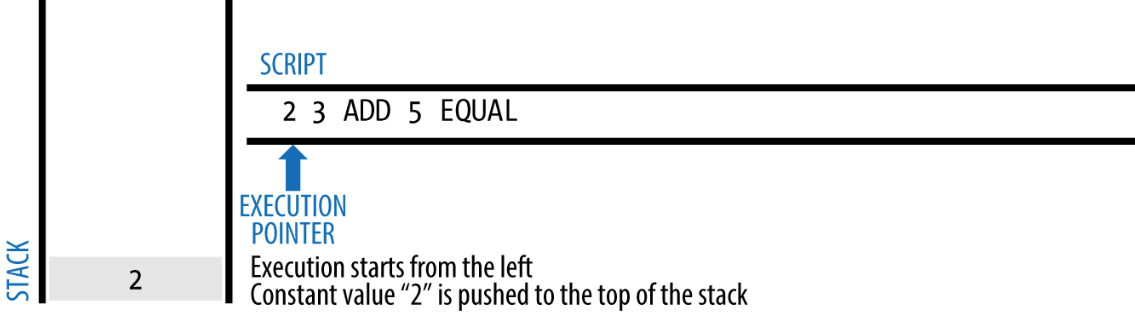
\includegraphics[width=\textwidth,clip=false]{pictures/stack1.png}}
    \only<2>{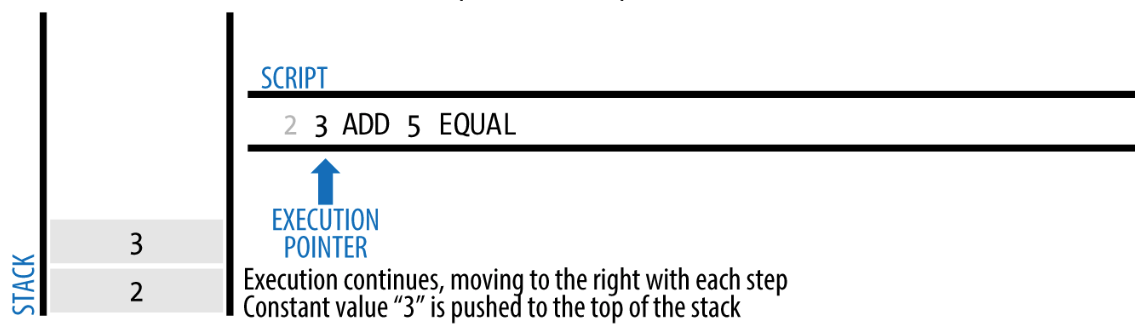
\includegraphics[width=\textwidth,clip=false]{pictures/stack2.png}}
    \only<3>{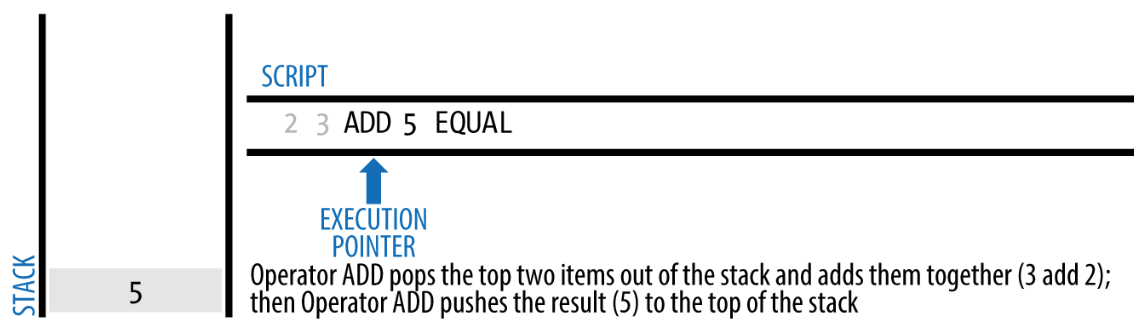
\includegraphics[width=\textwidth,clip=false]{pictures/stack3.png}}
    \only<4>{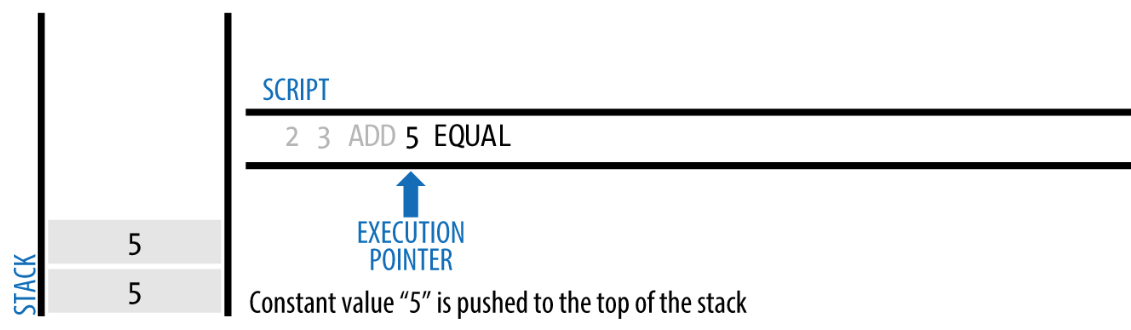
\includegraphics[width=\textwidth,clip=false]{pictures/stack4.png}}
    \only<5>{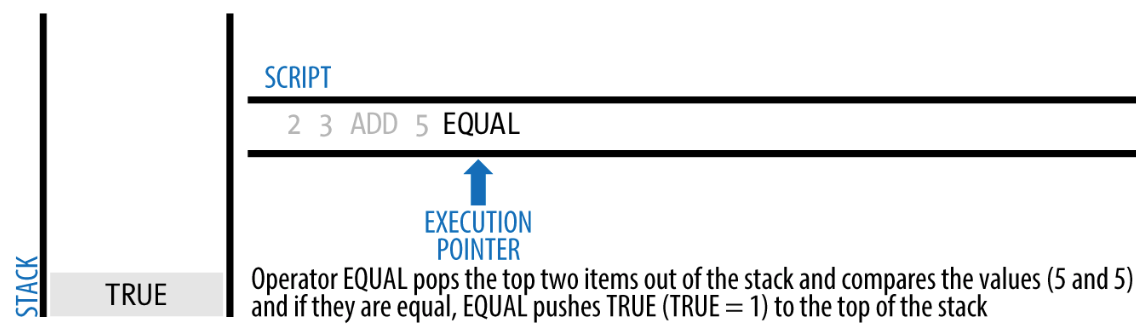
\includegraphics[width=\textwidth,clip=false]{pictures/stack5.png}}
  \end{center}

  \begin{center}
    \only<5>{The program is valid!}
  \end{center}

\end{frame}

\begin{frame}\frametitle{Other examples of (in-)valid scripts}

  \begin{greenbox}{These are all valid}
    \begin{itemize}
    \item \texttt{TRUE}
    \item \texttt{FALSE TRUE}
    \item \texttt{2 7 ADD 3 SUB 1 ADD 7 EQUAL}
    \item \texttt{2 7 EQUAL IF FALSE ELSE TRUE ENDIF}
    \end{itemize}
  \end{greenbox}

  \bigskip

  \begin{greenbox}{These are all invalid}
    \begin{itemize}
    \item \texttt{FALSE}
    \item \texttt{2 7 EQUAL}
    \item \texttt{2 7 EQUAL IF TRUE ELSE FALSE ENDIF}
    \item \texttt{2 7 EQUAL TRUE ENDIF}
    \end{itemize}
  \end{greenbox}

\end{frame}

\begin{frame}[fragile]\frametitle{The validation algorithm for bitcoin transactions}

{\scriptsize\begin{alltt}
previous_tx = \{ // this transaction has hash H
  "vins": .....
  "vouts": [ \{ "value": .....,     "lock": "....." \}, ..... ]
\}

tx = \{
  "vins": [ \{ "txid": H,     "vout": .....,     "unlock": "....." \}, ..... ],
  "vouts": .....
\}
\end{alltt}}

    {\small\begin{alltt}
    boolean is_valid(Transaction tx) \{
      for each (txid, vout, unlock) in tx.vins
        previous_tx = \alert{get_transaction}(txid)
        lock = previous_tx.vouts[vout].lock
        if ({\color{blue}{unlock lock}} is invalid)
          return false

      return true
    \}
    \end{alltt}}

\end{frame}

\begin{frame}[fragile]\frametitle{The typical P2PKH script (\emph{pay to publickey hash})}

\begin{greenbox}{``I want to send some value to \<address>''}
{\scriptsize\begin{alltt}
previous_tx = \{ // this transaction has hash H
  "vins": .....
  "vouts": [\{ "value": ..., "lock": {\color{blue}{DUP HASH160 <address> EQUALVERIFY CHECKSIG}} \},
            .....]
\}
\end{alltt}}
\end{greenbox}

\bigskip

\begin{greenbox}{``I'm \<address>, here is my signature, use that value''}
{\scriptsize\begin{alltt}
tx = \{
  "vins": [ \{ "txid": H,   "vout": .....,   "unlock": {\color{blue}{<sig> <PubK>}}\}, ..... ],
  "vouts": .....
\}
\end{alltt}}
\end{greenbox}

\bigskip

\begin{greenbox}{\<unlock lock>}
  \begin{center}
    \texttt{<sig> <PubK> DUP HASH160 <address> EQUALVERIFY CHECKSIG}
  \end{center}
\end{greenbox}

The bitcoin \<address> is often referred to as \<PublicKHash>

\end{frame}

\begin{frame}\frametitle{\texttt{<sig> <PubK> DUP HASH160 <address> EQUALVERIFY CHECKSIG}}

  \begin{center}
    \only<1>{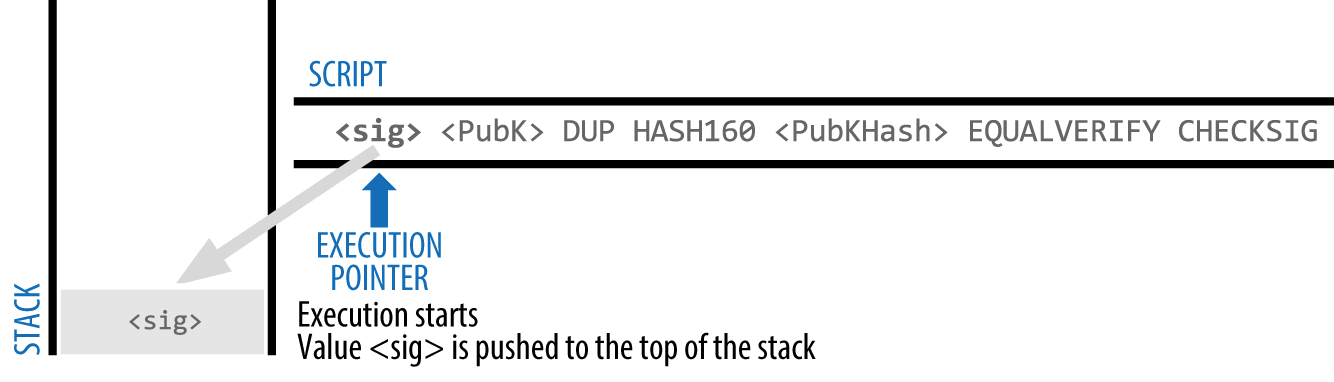
\includegraphics[width=\textwidth,clip=false]{pictures/p2pkh1.png}}
    \only<2>{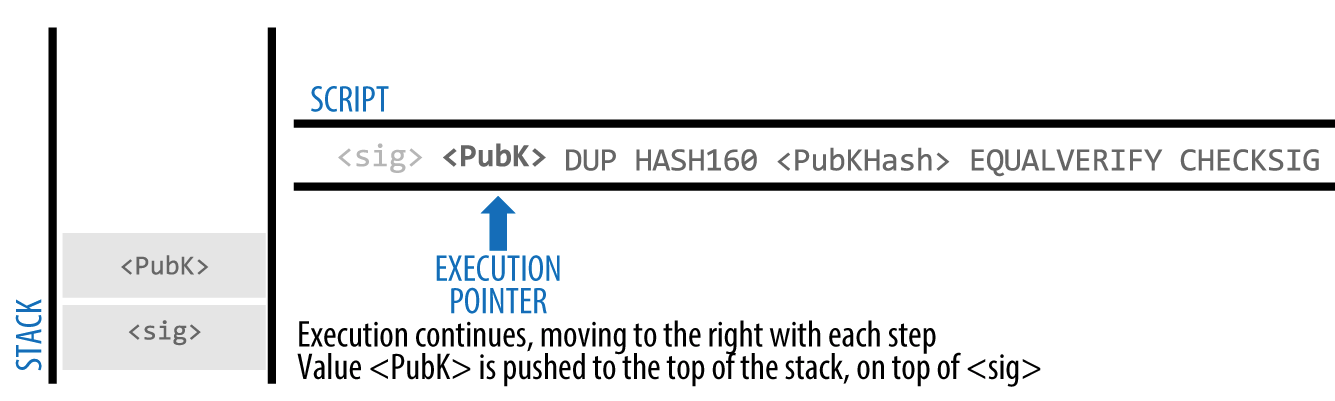
\includegraphics[width=\textwidth,clip=false]{pictures/p2pkh2.png}}
    \only<3>{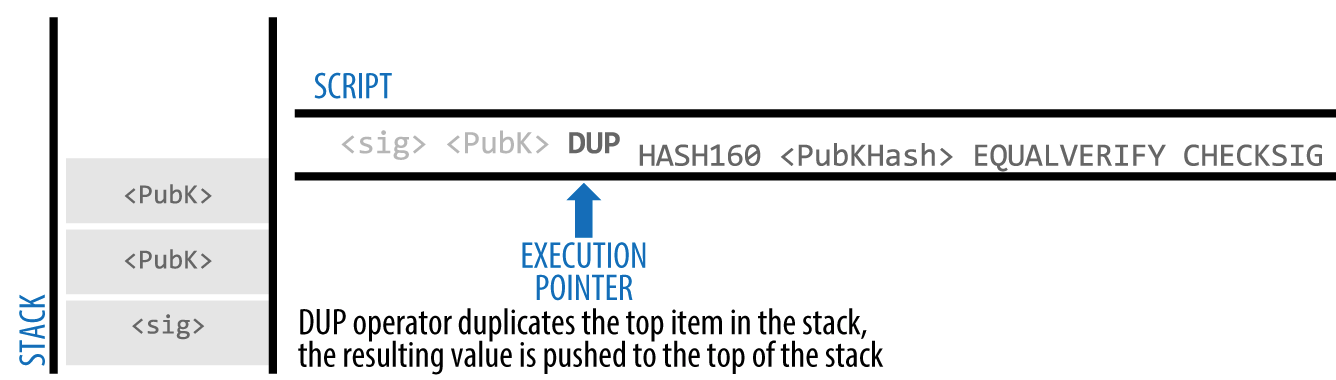
\includegraphics[width=\textwidth,clip=false]{pictures/p2pkh3.png}}
    \only<4>{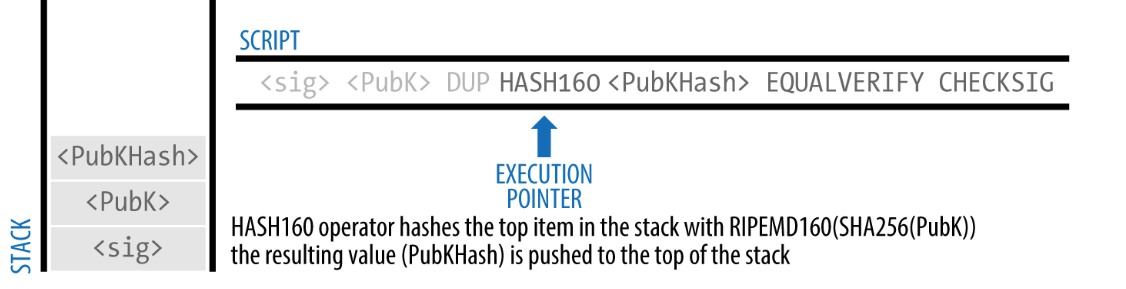
\includegraphics[width=\textwidth,clip=false]{pictures/p2pkh4.png}}
    \only<5>{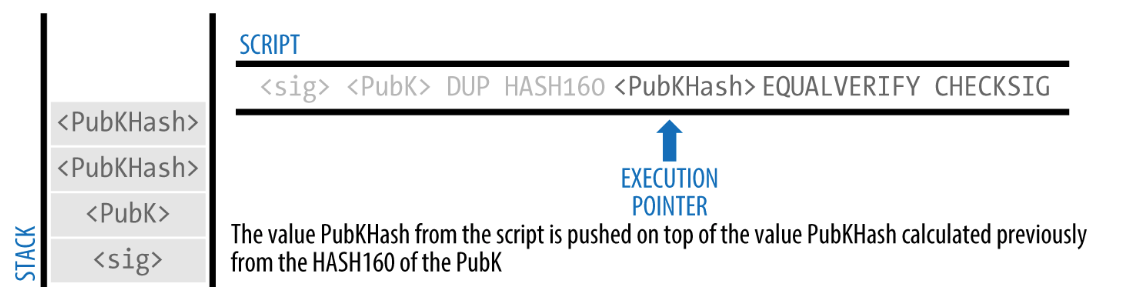
\includegraphics[width=\textwidth,clip=false]{pictures/p2pkh5.png}}
    \only<6-7>{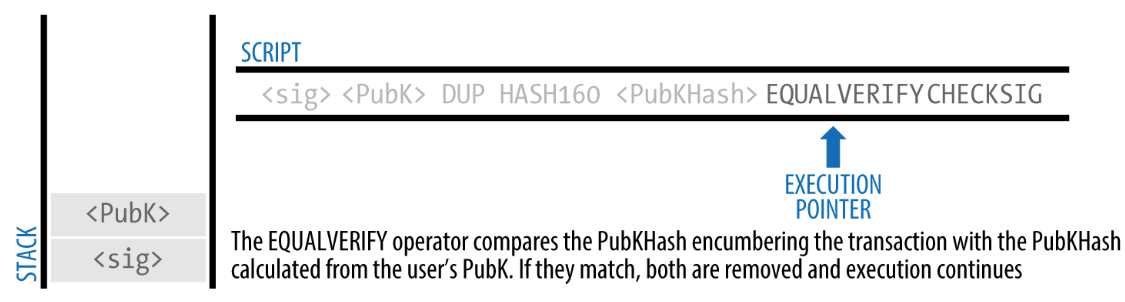
\includegraphics[width=\textwidth,clip=false]{pictures/p2pkh6.png}}+
    \only<8>{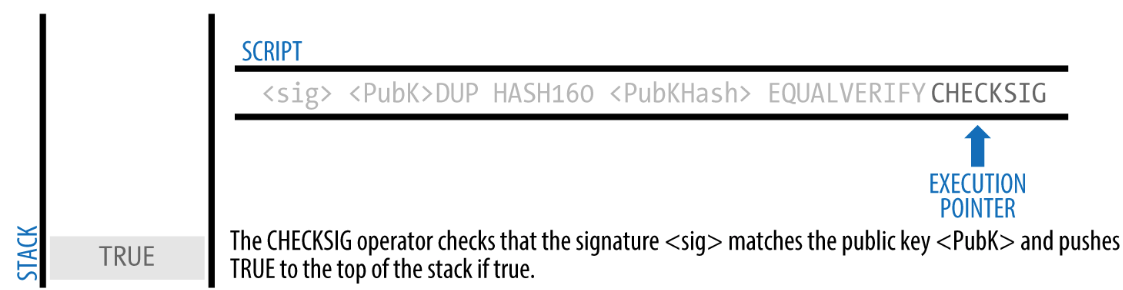
\includegraphics[width=\textwidth,clip=false]{pictures/p2pkh7.png}}
  \end{center}

  \uncover<7>{
    \begin{greenbox}{}
      \<CHECKSIG> verifies that \<sig> is a signature of the transaction
      by using the private key corresponsing to \<pubK>
    \end{greenbox}
  }

  \uncover<8>{
    \begin{center}
      This script gives proof of ownership!
    \end{center}
  }

\end{frame}

\begin{frame}[fragile]\frametitle{How block explorers and wallets infer accounts}

\begin{greenbox}{The typical transaction}
{\scriptsize\begin{alltt}
tx = \{
  "vins": [ \{ "txid": ..., "vout": ..., "unlock": {\color{blue}{<sig> <PubK>}}\}, ..... ],
  "vouts": [\{ "value": v, "lock": {\color{blue}{DUP HASH160 <address> EQUALVERIFY CHECKSIG}} \},
            .....]
\}
\end{alltt}}
\end{greenbox}

\bigskip

\begin{center}
  RIPEMD160(SHA256(\<PubK>)) $\xRightarrow[]{v}$ \<address>
\end{center}

\bigskip
\begin{redbox}{}
  \begin{center}
    Fragile! It works for the standard script only
  \end{center}
\end{redbox}

\end{frame}

\begin{frame}\frametitle{Headers, blocks and blockchain, genesis block}

  \begin{center}
    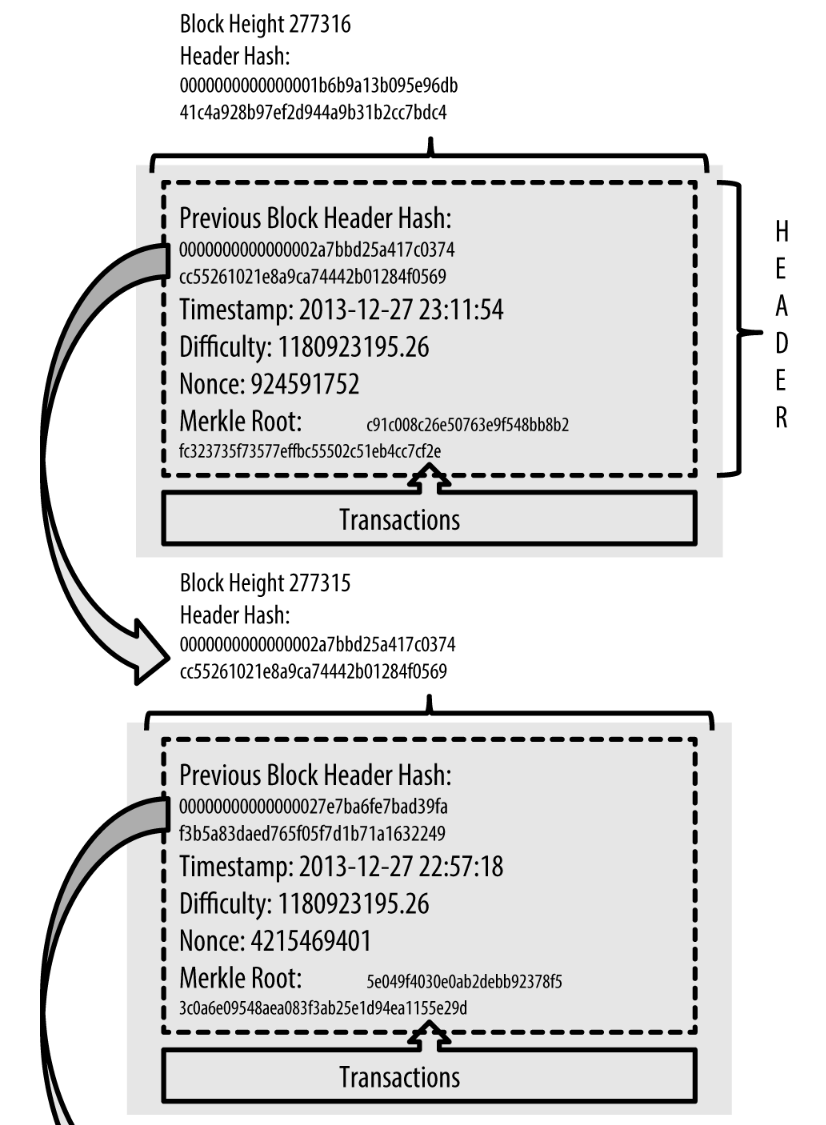
\includegraphics[scale=0.2,clip=false]{pictures/bitcoin-blocks.png}
  \end{center}

\end{frame}

\begin{frame}\frametitle{The blockchain grows}

  \begin{greenbox}{Full nodes are peers that keep the full blockchain in their database}
    \begin{itemize}
    \item they receive transactions from other peers or the outside world
      \begin{itemize}
      \item they keep them in their mempool
      \item they whisper them to their peers
      \end{itemize}
    \item they produce blocks by packing mempool transactions
      \begin{itemize}
      \item they forward them to their peers
      \end{itemize}
    \item they receive blocks from peers
      \begin{itemize}
      \item they use the previous block hash of the received blocks to
        attach them at the right place in the blockchain

        $\Rightarrow$ the bitcoin blockchain is a tree, not a list
      \end{itemize}
    \end{itemize}
  \end{greenbox}

\end{frame}

\begin{frame}\frametitle{The header contains the hash of the transactions (Merkle root)}

  \begin{center}
    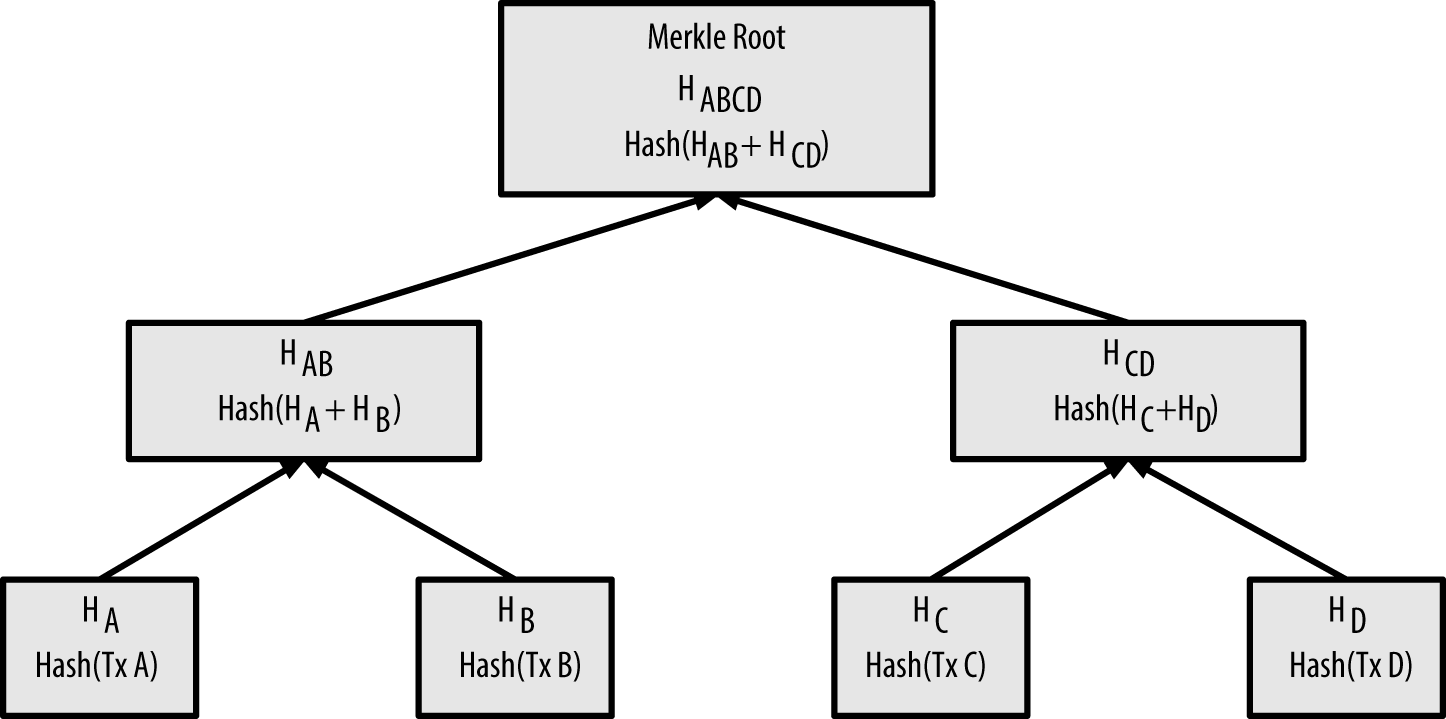
\includegraphics[width=\textwidth,clip=false]{pictures/mbc2_0902.png}
  \end{center}

\end{frame}

\begin{frame}\frametitle{Merkle trees provide an efficient inclusion test}

  \begin{center}
    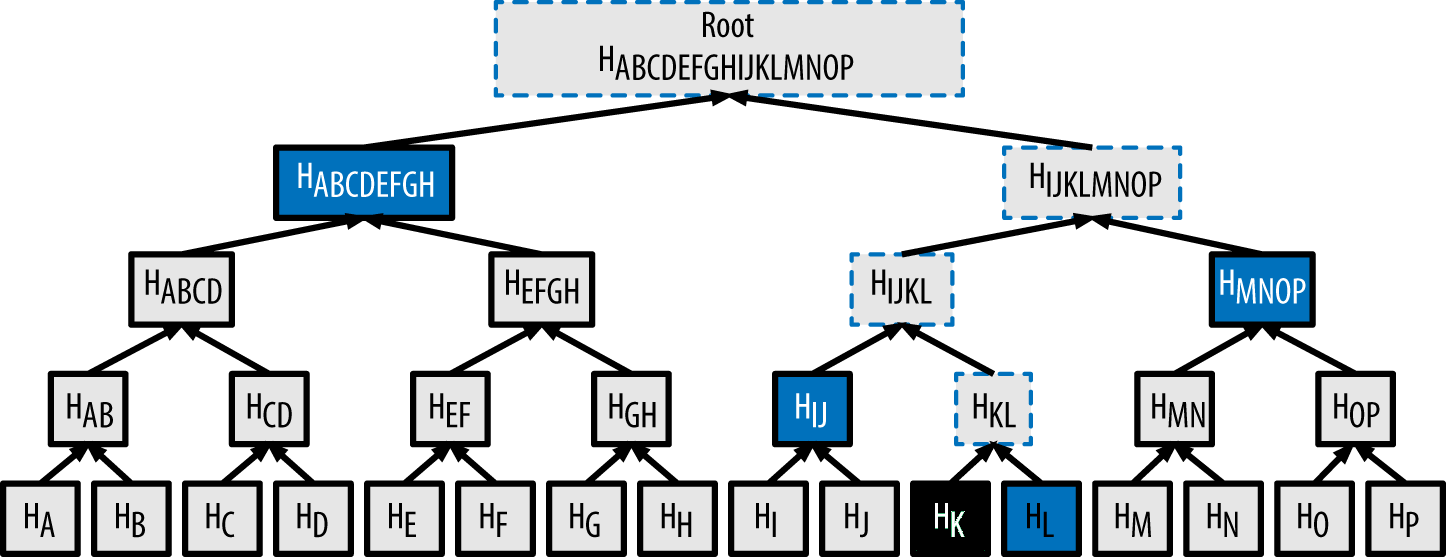
\includegraphics[width=\textwidth,clip=false]{pictures/mbc2_0905.png}
  \end{center}

  \begin{greenbox}{I know the root hash and want to know if the {\color{black}black $H_K$} is included}
    The {\color{blue}four blue hashes} can be given to me as that proof of inclusion
    (\emph{authentication path})
  \end{greenbox}

\end{frame}

\begin{frame}\frametitle{The Merkle tree helps external tools}

  \begin{greenbox}{A wallet wants to know when its transaction $t$ has been processed}
    \begin{itemize}
    \item the wallet downloads the header of each new block from a full node;
      the header is much smaller than the block; it contains the Merkle tree's root
    \item the wallet asks the full node for a proof of inclusion of $t$ in the block
    \item the full node answers with a proof consisting of only
      $32\times\log_2(\mathit{transactions\_in\_block})$ bytes
    \item the wallet checks the proof by computing
      $\log_2(\mathit{transactions\_in\_block})$ hashes and comparing the last
      hash computed to the Merkle root in the header
    \end{itemize}
  \end{greenbox}

\end{frame}

\begin{frame}\frametitle{The Merkle tree is not in blockchain!}

  \begin{greenbox}{}
    \begin{itemize}
    \item it is not in the blocks
    \item it is not in the header of the blocks
      \begin{itemize}
      \item[$\Rightarrow$] only the hash of the Merkle tree's root is in the header
      \end{itemize}
    \item it is in the volatile memory of full nodes
      \begin{itemize}
      \item[$\Rightarrow$] to answer inclusion tests with a short, efficient proof
      \end{itemize}      
    \end{itemize}
  \end{greenbox}

  \bigskip

  \begin{center}
    
\includegraphics[scale=0.5,clip=false]{pictures/ghost-tree.png}
  \end{center}

\end{frame}

\begin{frame}\frametitle{Mining}

  \begin{center}
    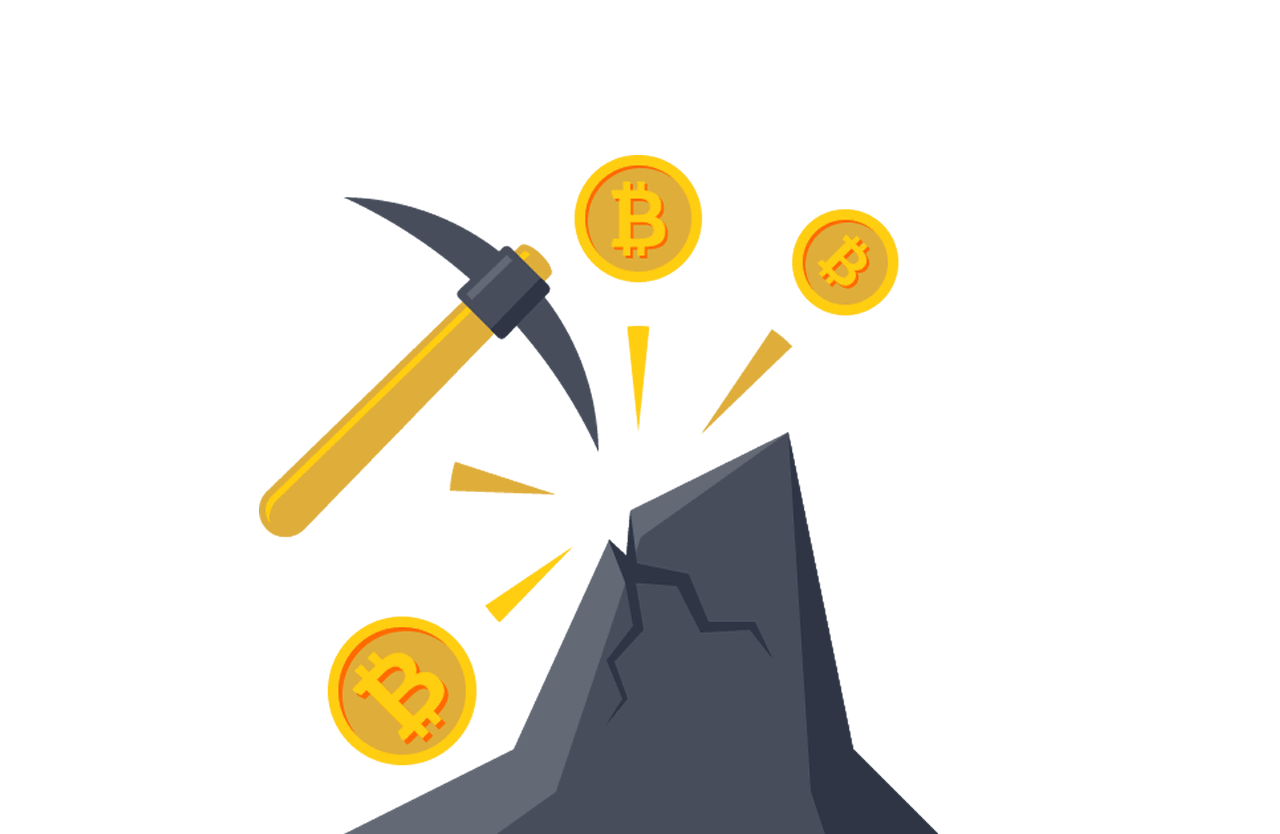
\includegraphics[scale=0.1,clip=false]{pictures/mining.png}
  \end{center}

  \bigskip

  \begin{greenbox}{The vision of the miner}
    The goal of mining is to mint new coins and earn money
  \end{greenbox}

  \bigskip

  \begin{greenbox}{The vision of Nakamoto}
    The goal of mining is to secure the bitcoin network
  \end{greenbox}

\end{frame}

\begin{frame}\frametitle{Miners are expected to create new \emph{valid} blocks}

  \begin{greenbox}{New valid block = it respects the {\color{pink}{consensus rules}}}
    \begin{itemize}
    \item the structure of data in the header and transactions must be correct
    \item transactions have at least one input (but for coinbase transactions)
    \item transactions have at least one output
    \item transactions do not create money (but for coinbase transactions)
    \item coinbase transactions have a correct reward
    \item transactions are all valid (their unlocking scripts match the corresponsing locking scripts)
    \item transaction inputs refer to unspent UTXO only
      (\alert{no double-spending inside the same history})
    \item \ldots
    \end{itemize}
  \end{greenbox}
  
\end{frame}

\begin{frame}\frametitle{Construction of a new valid block at height $H$}

    \begin{greenbox}{}
      \begin{itemize}
      \item addition of a selection of some valid transactions from the mempool
      \item addition of a coinbase transaction
      \item computation of their Merkle tree root
      \item creation of the block's header:
        \begin{itemize}
        \item hash of block $H-1$
        \item timestamp
        \item Merkle tree root
        \item nonce (for now, an arbitrary number)
        \end{itemize}
      \end{itemize}
    \end{greenbox}

    \bigskip

    \begin{greenbox}{If a miner receives from its peers a block $b$ at height $H$
        while it's building that same block}
      It verifies the validity of $b$. If $b$ is valid,
      it stops working at the block at height $H$, adds $b$ to the blockchain,
      considers the inputs of the transactions in $b$ as spent,
      and immediately starts working at block at height $H+1$ on top of $b$. In this sense,
      the miner \emph{votes} for $b$
    \end{greenbox}

\end{frame}

\begin{frame}\frametitle{Whom should I trust?}

  \begin{redbox}{The construction of a new block is too easy!}
    Just a small fraction of a second

    \begin{itemize}
    \item[$\Rightarrow$] each miner can build as many blocks as it wants
    \item[$\Rightarrow$] each miner can decide its own history
    \end{itemize}
  \end{redbox}

  \bigskip
  \bigskip

  \pause

  \begin{center}
    The real genius of Nakamoto:\\

    \mbox{}\\
    
    {\Huge make it randomly hard!}
  \end{center}

\end{frame}

\begin{frame}\frametitle{Proof-of-work (PoW)}

  \begin{greenbox}{Add the following consensus rule}
    The hash of valid blocks is smaller than
    a given constant $\mathit{difficulty}$
  \end{greenbox}

  \bigskip

  \begin{greenbox}{Each miner does some work}
    \begin{enumerate}
    \item build a new block
    \item set the nonce field of its header to a random value
    \item compute the hash $h$ of the header
    \item if $h < \mathit{difficulty}$ stop
    \item go back to step 2
    \end{enumerate}
  \end{greenbox}

  \bigskip

  \begin{itemize}
  \item the nonec in the header of the resulting block is the PoW
  \item the time to solve this puzzle is inversely proportional to $\mathit{difficulty}$
  \item the algorithm can be easily run in parallel
  \end{itemize}

\end{frame}

\begin{frame}\frametitle{The blockchain grows}

  \begin{itemize}
  \item the miner creates a new block on top of the main history
  \item the miner receives a valid new block from a peer
    \begin{itemize}
    \item whose parent is the top of the main history, or
    \item whose parent is another block of the blockchain (fork), or
    \item whose parent is unknown to the miner (orphan block)
    \end{itemize}
  \item in case of fork, the main history is the longest one (actually: the most powerful one), but the miner keeps all histories,
    in case they might become the new main history in the future
  \end{itemize}

  \[
  \mathit{power}(\mathit{chain})=\sum_{\mathit{block}\in\mathit{chain}}\frac{2^{8\cdot 32}}{\mathit{block}.\mathit{nonce}+1}
  \]
\end{frame}

\begin{frame}\frametitle{Fork: all nodes start with the same vision}

  \begin{center}
    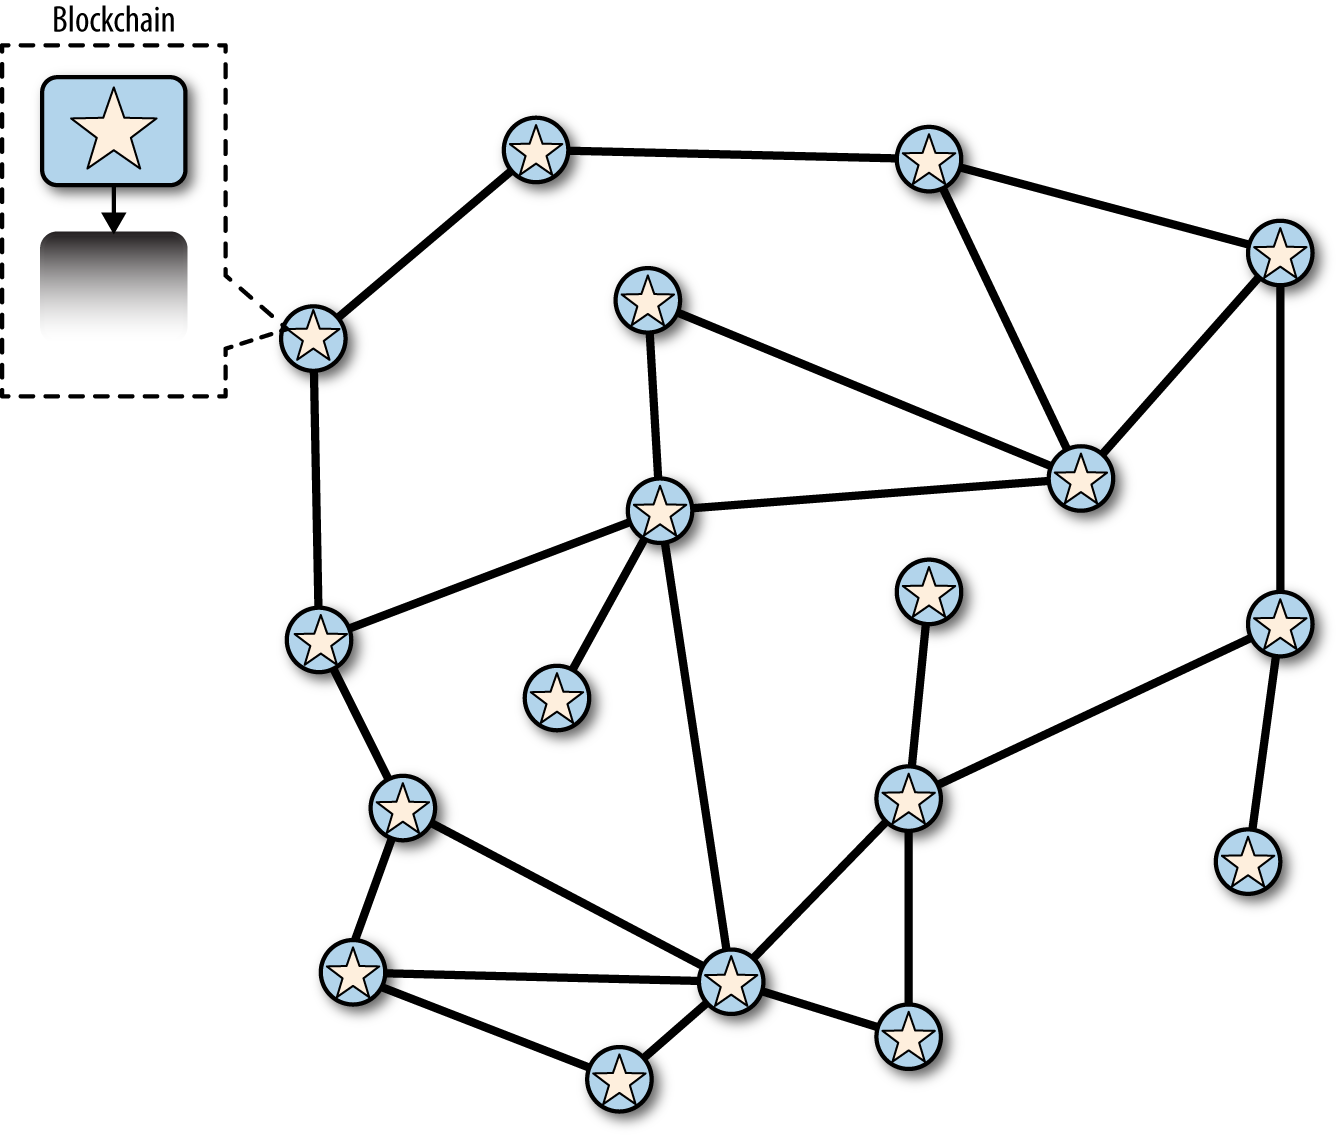
\includegraphics[scale=0.8,clip=false]{pictures/mbc2_1002.png}
  \end{center}

\end{frame}

\begin{frame}\frametitle{Fork: two nodes expand the blockchain simultaneously}

  \begin{center}
    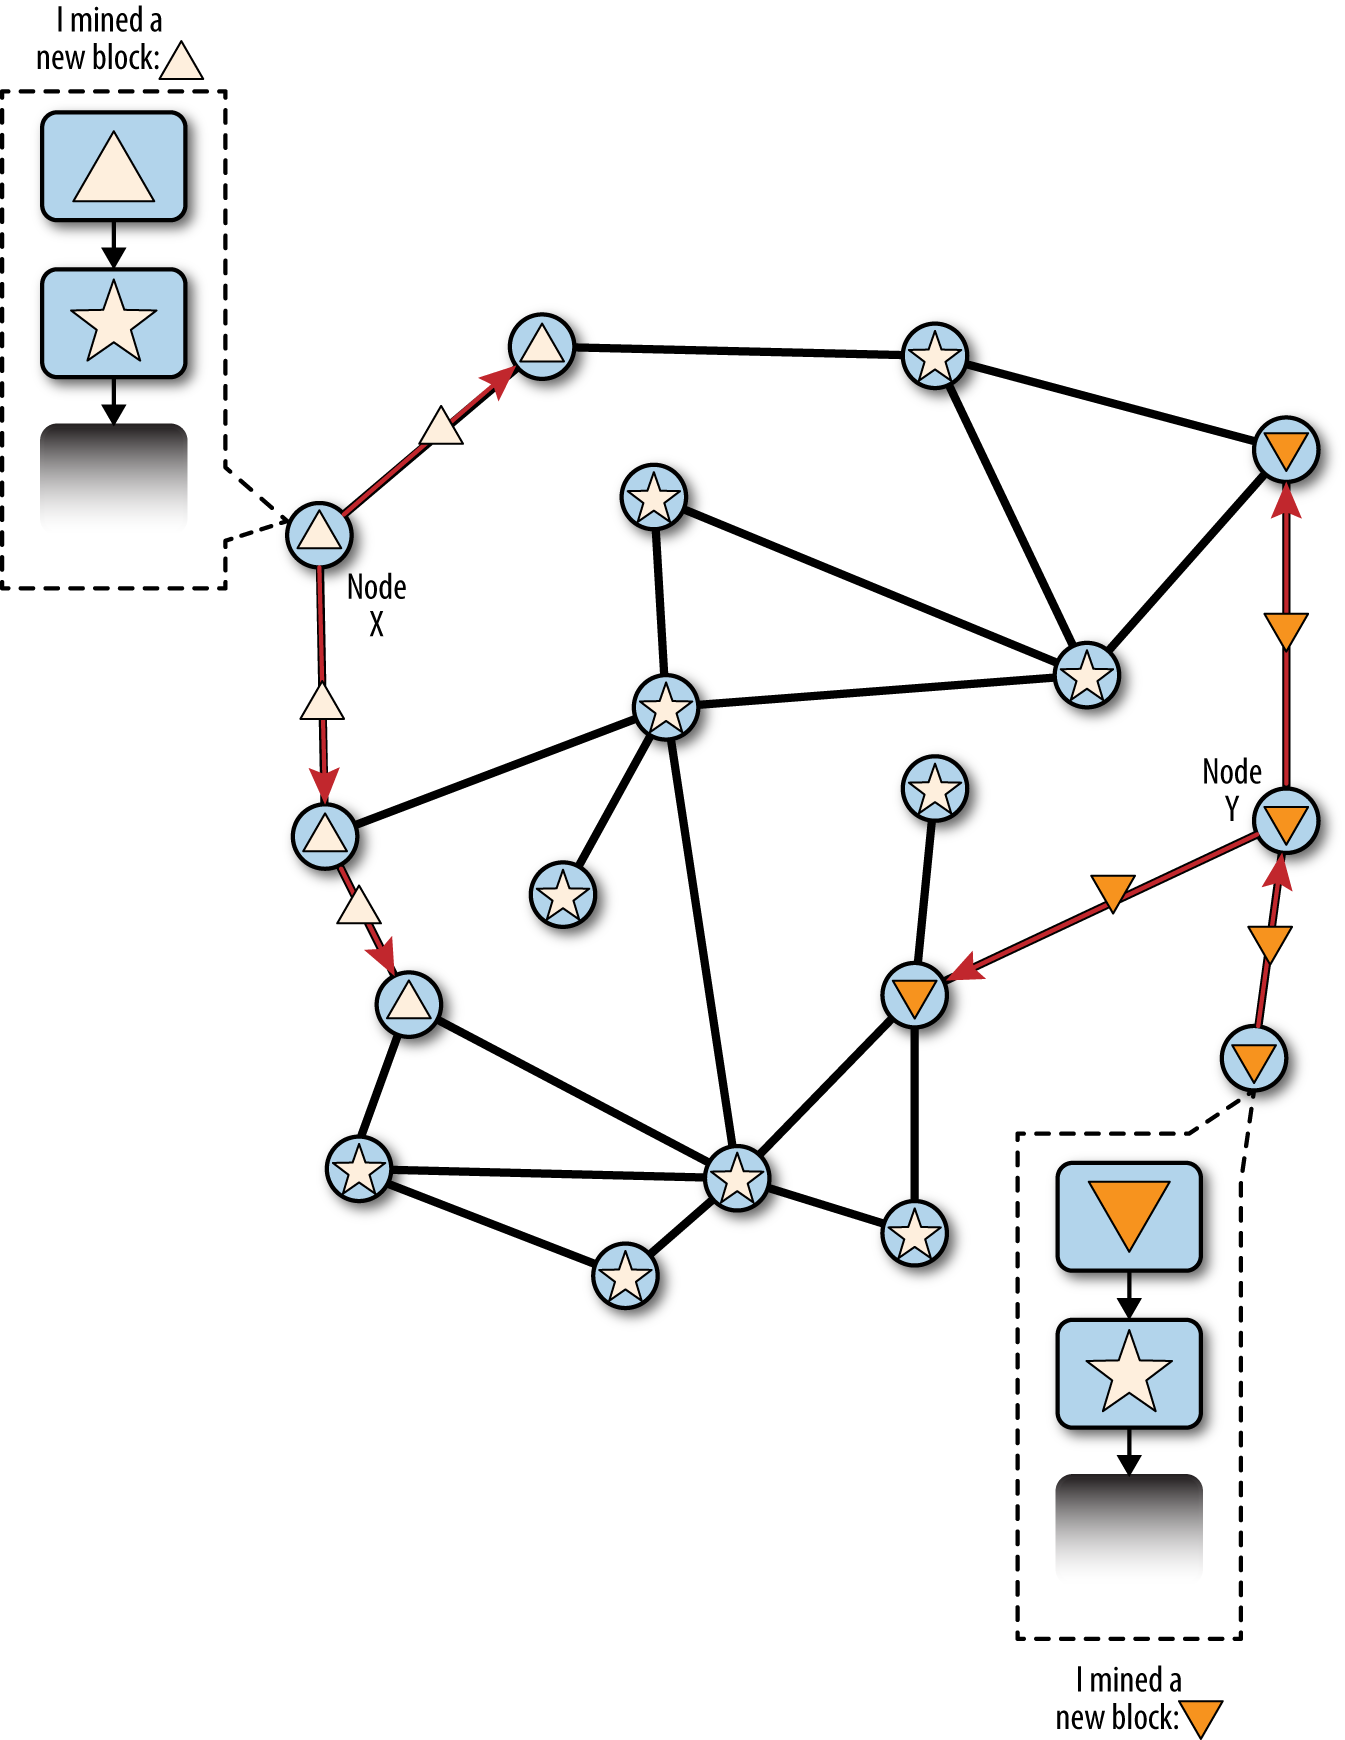
\includegraphics[scale=0.53,clip=false]{pictures/mbc2_1003.png}
  \end{center}

\end{frame}

\begin{frame}\frametitle{Fork: the network is split}

  \begin{center}
    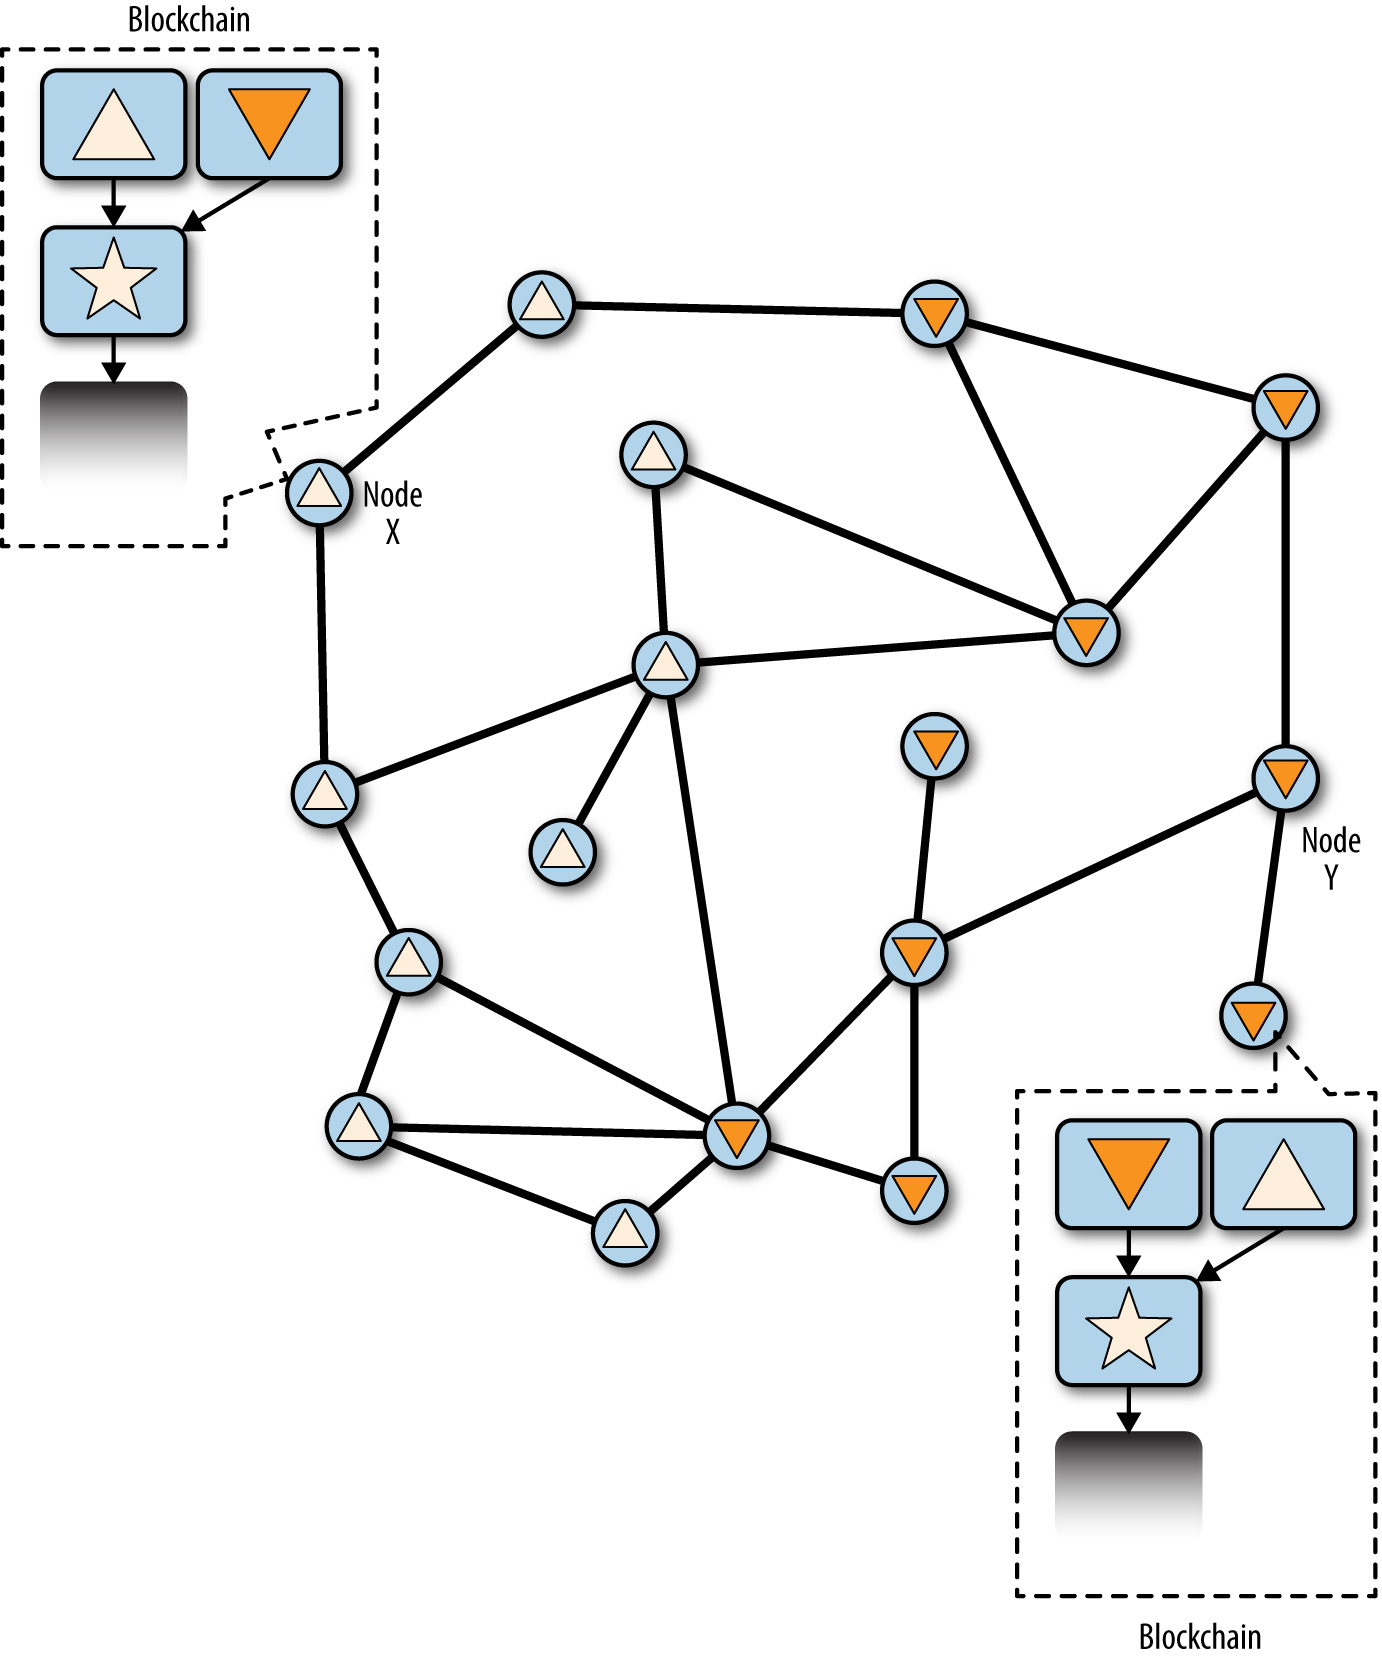
\includegraphics[scale=0.56,clip=false]{pictures/mbc2_1004.png}
  \end{center}

\end{frame}

\begin{frame}\frametitle{Fork: either chain is expanded further}

  \begin{center}
    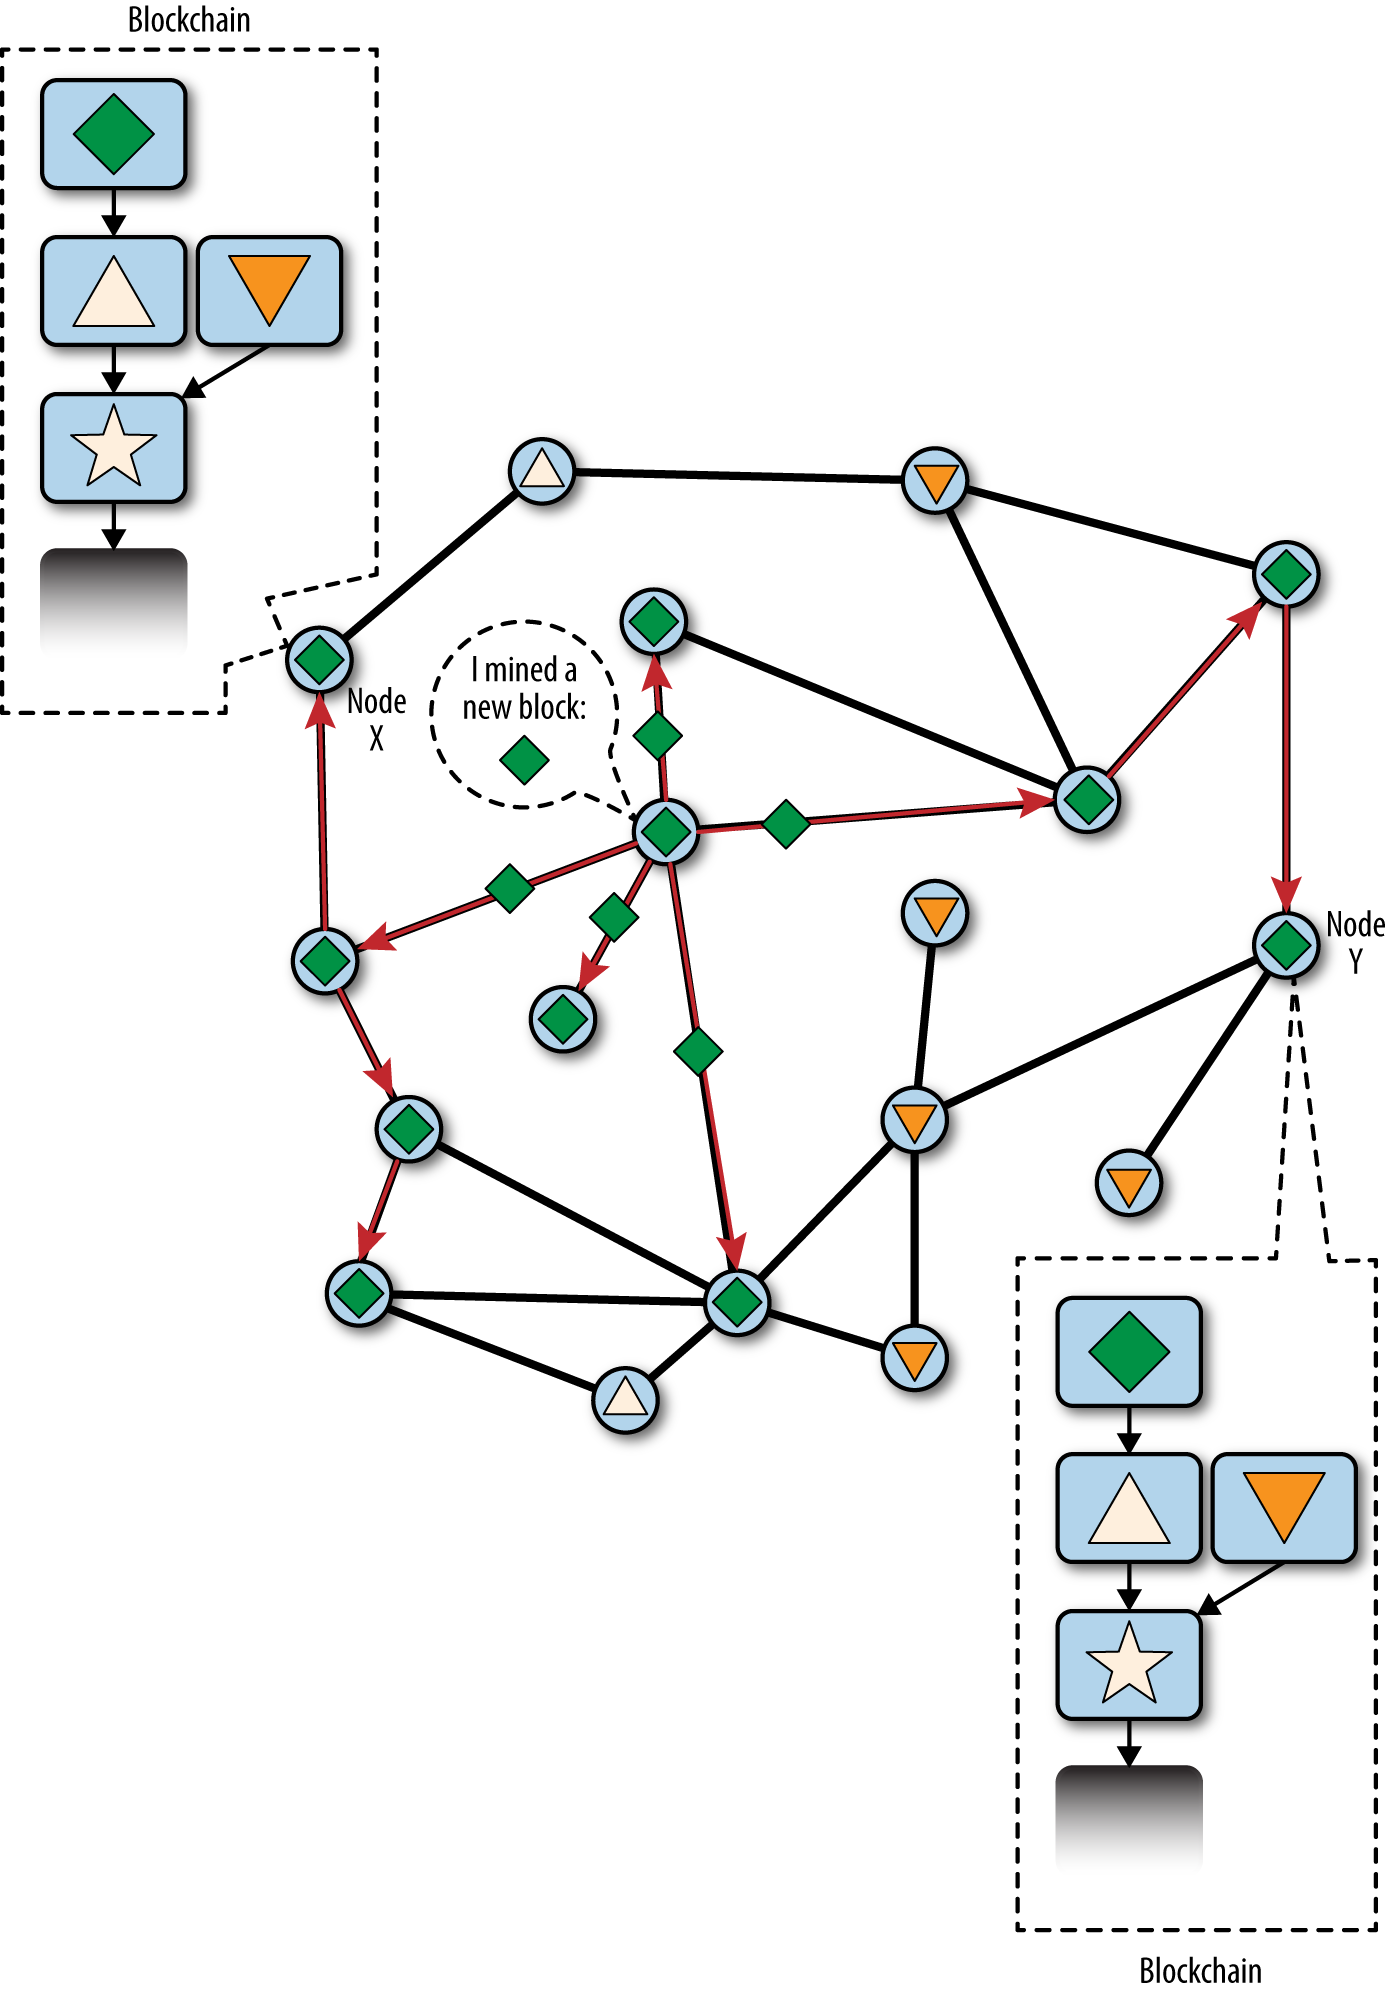
\includegraphics[scale=0.47,clip=false]{pictures/mbc2_1005.png}
  \end{center}

\end{frame}

\begin{frame}\frametitle{Fork: the network reconverges}

  \begin{center}
    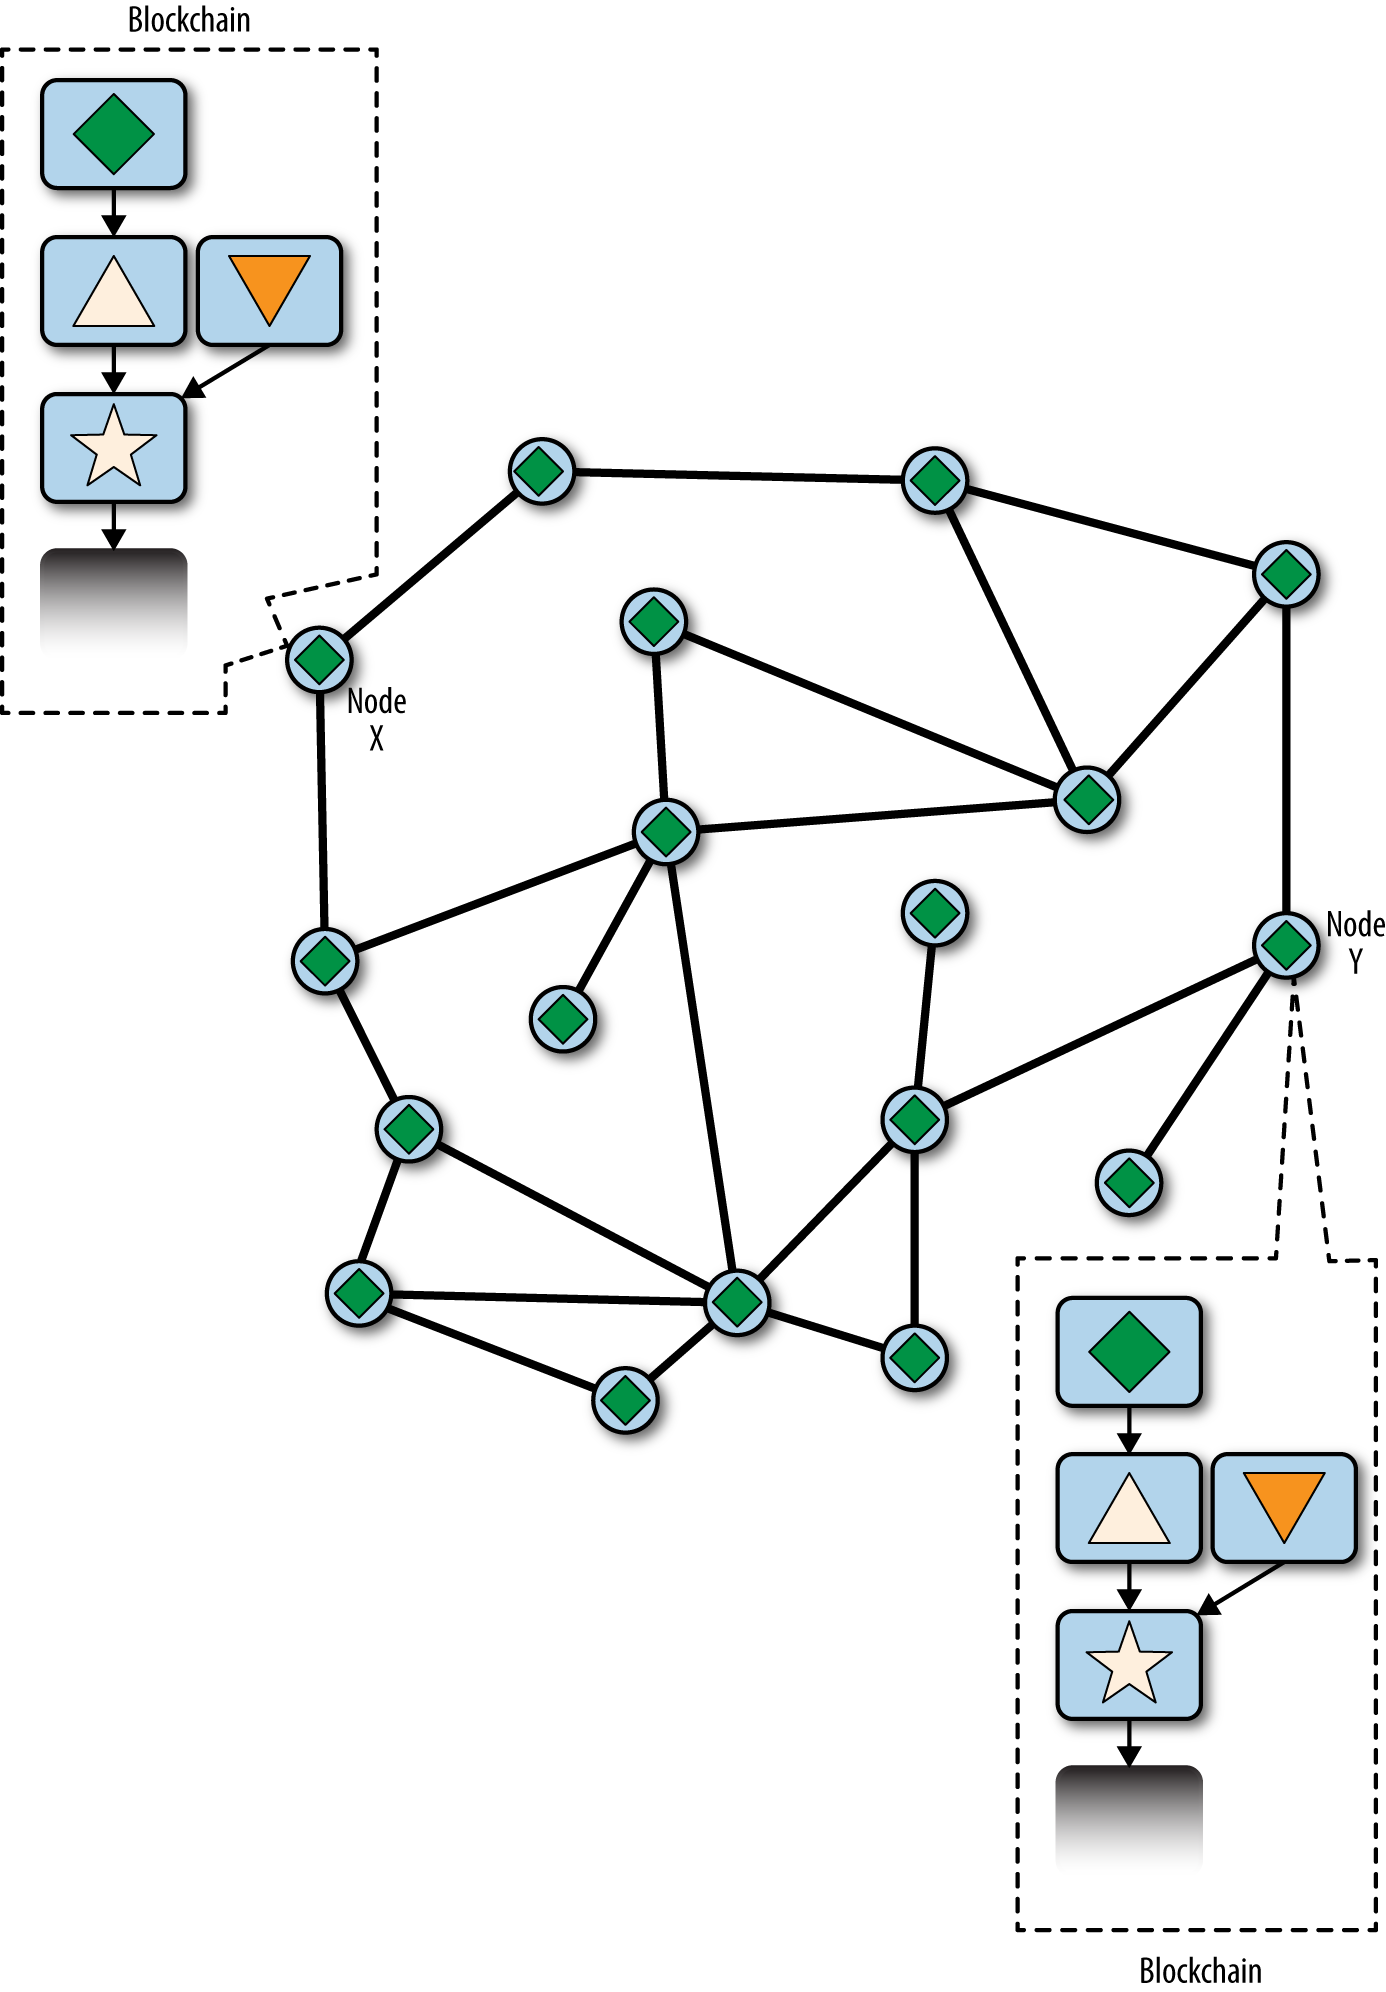
\includegraphics[scale=0.47,clip=false]{pictures/mbc2_1006.png}
  \end{center}

\end{frame}

\begin{frame}\frametitle{The magic behind PoW}

  \begin{greenbox}{}
    It makes expensive the production of new blocks, in time and cost (electricity)
    \begin{itemize}
    \item who produces invalid blocks sees its blocks rejected by peers and wastes resources
    \item a single node cannot drive the history, since it must fight against
      the hashing power of all other nodes together
    \item forks become unlikely, since the probability of finding a new block at the same time
      is small
    \end{itemize}
  \end{greenbox}

\end{frame}

\begin{frame}\frametitle{Difficulty over time}

  \begin{center}
    \includegraphics[width=\textwidth,clip=false]{pictures/difficulty.jpg}
  \end{center}

\end{frame}

\begin{frame}\frametitle{PoW costs electricity}

  \begin{greenbox}{2019}
    \begin{center}
      \includegraphics[scale=0.17,clip=false]{pictures/bitcoin-consumption.jpg}
      \includegraphics[scale=0.14,clip=false]{pictures/greta.jpg}
    \end{center}
  \end{greenbox}
    
\end{frame}

\begin{frame}\frametitle{Consensus attacks}

  \begin{greenbox}{Two main categories}
    \begin{enumerate}
    \item history change (for the topmost few blocks)
    \item denial-of-service (against specific transactions or accounts)
    \end{enumerate}
  \end{greenbox}

  \bigskip

  Possible if the attacker controls a large portion of the total hashing power

  \begin{center}
    \includegraphics[scale=0.17,clip=false]{pictures/51-percenters.jpg}
  \end{center}

\end{frame}

\begin{frame}\frametitle{How the 51\% attack works}

  \begin{greenbox}{The malicious miner spends $100$ BTC on the public chain
      while it is adding blocks to its
      private blockchain, without broadcasting them. In its private chain,
      the spend transaction is missing}
    \begin{center}
      \includegraphics[width=\textwidth,clip=false]{pictures/51attack_1.png}
    \end{center}
  \end{greenbox}

\end{frame}

\begin{frame}\frametitle{How the 51\% attack works}

  \begin{greenbox}{The malicious miner makes its private chain longer,
      since it has more hashing power than the rest of the miners taken together}
  \begin{center}
    \includegraphics[width=\textwidth,clip=false]{pictures/51attack_2.png}
  \end{center}
  \end{greenbox}

\end{frame}

\begin{frame}\frametitle{How the 51\% attack works}

  \begin{greenbox}{The malicious miner broadcasts its private chain; since it is longer,
      all other miners switch to this alternative view of the history}
  \begin{center}
    \includegraphics[width=\textwidth,clip=false]{pictures/51attack_3.png}
  \end{center}
  \end{greenbox}

\end{frame}

\begin{frame}\frametitle{How the 51\% attack works}

  \begin{greenbox}{The malicious miner can spend its $100$ BTC again! Everybody agrees\ldots}
  \begin{center}
    \includegraphics[width=\textwidth,clip=false]{pictures/51attack_4.png}
  \end{center}
  \end{greenbox}

  \bigskip

  \begin{center}
    History is written by the victors
  \end{center}

\end{frame}

\begin{frame}\frametitle{Bitcoin has probabilistic finality}

  \begin{center}
    \includegraphics[width=\textwidth,clip=false]{pictures/finality.png}
  \end{center}

\end{frame}

\begin{frame}\frametitle{Changing the consensus rules}

  \begin{greenbox}{Why?}
    \begin{itemize}
    \item new features
    \item bug fixes
    \item protocols exist for voting for/against the upgrade, before the new rules
      get activated
    \end{itemize}
  \end{greenbox}

\end{frame}

\begin{frame}\frametitle{Soft fork: new rules more restrictive than old rules}

  \begin{greenbox}{}
    \begin{itemize}
    \item if the next block is mined by a yellow node, it is accepted by all nodes
    \item if the next block is mined by a black node, it might be rejected by the yellow nodes
    \item if at least $51\%$ of the hashing power is yellow (upgraded), the network will not split and will follow
      the new rules of the yellow nodes
    \end{itemize}
  \end{greenbox}

  \bigskip

  \begin{center}
    \includegraphics[width=\textwidth,clip=false]{pictures/soft-fork.png}
  \end{center}

\end{frame}

\begin{frame}\frametitle{Hard fork: new rules less restrictive than old rules}

  \begin{redbox}{}
    \begin{itemize}
    \item if the next block is mined by a black node, it is accepted by all nodes
    \item if the next block is mined by a yellow node, it might be rejected by the black nodes
    \item if at least $51\%$ of the hashing power is yellow (upgraded), the network splits in two
    \end{itemize}
  \end{redbox}

  \bigskip

  \begin{center}
    \includegraphics[width=\textwidth,clip=false]{pictures/hard-fork.png}
  \end{center}
    
\end{frame}

\end{document}
